% Guides
% http://ivk.knteu.kiev.ua/docum/z_vg.pdf
% http://www.ivk.knteu.kiev.ua/docum/prav01.pdf
\documentclass[a4paper,14pt,oneside,final]{extarticle}
\usepackage[top=2cm, bottom=2cm, left=3cm, right=1cm]{geometry}
\usepackage{scrextend}

\usepackage[T2A,T1]{fontenc}
\usepackage[ukrainian,russian,english]{babel}
\usepackage{tempora}
\usepackage{fontspec}
\setmainfont{tempora}

% Зачем: Отключает использование изменяемых межсловных пробелов.
% Почему: Так не принято делать в текстах на русском языке.
\frenchspacing

\usepackage{indentfirst}
\setlength{\parindent}{1.25cm}
\renewcommand{\baselinestretch}{1.5}

% Header
\usepackage{fancyhdr}
\pagestyle{fancy}
\fancyhead{}
\fancyfoot{}
\fancyhead[R]{\small \selectfont \thepage}
\renewcommand{\headrulewidth}{0pt}

% Captions
\usepackage{chngcntr}
\counterwithin{figure}{section}
\counterwithin{table}{section}
\usepackage[tableposition=top]{caption}
\usepackage{subcaption}
\DeclareCaptionLabelFormat{gostfigure}{Рисунок #2}
\DeclareCaptionLabelFormat{gosttable}{Таблиця #2}
\DeclareCaptionLabelSeparator{gost}{~---~}
\captionsetup{labelsep=gost}
\captionsetup[figure]{labelformat=gostfigure}
\captionsetup[table]{labelformat=gosttable}
\renewcommand{\thesubfigure}{\asbuk{subfigure}}

% Sections
\usepackage[explicit]{titlesec}
\newcommand{\sectionbreak}{\clearpage}

\titleformat{\section}
  {\centering}{\thesection \quad}{0pt}{\MakeUppercase{#1}}
\titleformat{\subsection}[block]
  {\bfseries}{\thesubsection \quad #1}{0cm}{}

\titlespacing{\section} {0cm}{0cm}{21pt}
\titlespacing{\subsection} {\parindent}{21pt}{0cm}
\titlespacing{\subsubsection} {\parindent}{0cm}{0cm}

% Lists
\usepackage{enumitem}
\renewcommand\labelitemi{--}
\setlist[itemize]{noitemsep, topsep=0pt, wide}
\setlist[enumerate]{noitemsep, topsep=0pt, wide, label=\arabic*}
\setlist[description]{labelsep=0pt, noitemsep, topsep=0pt, leftmargin=2\parindent, labelindent=\parindent, labelwidth=\parindent, font=\normalfont}

% Toc
\usepackage{tocloft}
\tocloftpagestyle{fancy}
\renewcommand{\cfttoctitlefont}{}
\setlength{\cftbeforesecskip}{0pt}
\renewcommand{\cftsecfont}{}
\renewcommand{\cftsecpagefont}{}
\renewcommand{\cftsecleader}{\cftdotfill{\cftdotsep}}

\usepackage{float}
\usepackage{pgfplots}
\usepackage{graphicx}
\usepackage{multirow}
\usepackage{amssymb,amsfonts,amsmath,amsthm}
\usepackage{csquotes}

\usepackage{listings}
\lstset{basicstyle=\footnotesize\ttfamily,breaklines=true}
\lstset{language=Matlab}

\usepackage[
	backend=biber,
	sorting=none,
	language=auto,
	autolang=other
]{biblatex}
\DeclareFieldFormat{labelnumberwidth}{#1}

% Copied from
% https://github.com/cansik/kotlin-latex-listing
% big thanks to him!
\lstdefinelanguage{Kotlin}{
  keywords={package, as, as?, typealias, this, super, val, var, fun, for, null, true, false, is, in, throw, return, break, continue, object, if, try, else, while, do, when, class, interface, enum, object, companion, override, public, private, get, set, import, abstract, vararg, expect, actual, where, suspend, data, internal, dynamic, final, by},
  keywordstyle=\color{NavyBlue}\bfseries,
  ndkeywords={@Deprecated, @JvmName, @JvmStatic, @JvmOverloads, @JvmField, @JvmSynthetic, Iterable, Int, Long, Integer, Short, Byte, Float, Double, String, Runnable, Array},
  ndkeywordstyle=\color{BurntOrange}\bfseries,
  emph={println, return@, forEach, map, mapNotNull, first, filter, firstOrNull, lazy, delegate},
  emphstyle={\color{OrangeRed}},
  identifierstyle=\color{black},
  sensitive=true,
  commentstyle=\color{gray}\ttfamily,
  comment=[l]{//},
  morecomment=[s]{/*}{*/},
  stringstyle=\color{ForestGreen}\ttfamily,
  morestring=[b]",
  morestring=[s]{"""*}{*"""},
}


\usepackage{lastpage}
\usepackage{calc}
\usepackage{soul}
\usepackage{pbox}
\usepackage{ulem}
\usepackage{titling}
\usepackage{framed}
\usepackage{tabu}
\usepackage{appendix}
\usepackage{packages/tikz-uml}
\usepackage[nomain,acronym,toc,nogroupskip,sort=def,xindy={glsnumbers=false}]{glossaries}
\usepackage[figure,table]{totalcount}

\makeglossaries
\newglossarystyle{mylist}{%  
 % put the glossary in the itemize environment:  
 \renewenvironment{theglossary}%  
   {\begin{itemize}[label={}]}{\end{itemize}}%  
 % have nothing after \begin{theglossary}:  
 \renewcommand*{\glossaryheader}{}%  
 % have nothing between glossary groups:  
 \renewcommand*{\glsgroupheading}[1]{}%  
 \renewcommand*{\glsgroupskip}{}%  
 % set how each entry should appear:  
 \renewcommand*{\glossentry}[2]{%  
 \item % bullet point  
 \glstarget{##1}{\glossentryname{##1}}% the entry name  
 \space ---% the symbol in brackets  
 \space \glossentrydesc{##1}% the description  
 %\space [##2]% the number list in square brackets
 .  
 }%  
 % set how sub-entries appear:  
 \renewcommand*{\subglossentry}[3]{%  
   \glossentry{##2}{##3}}%  
 } 
\setglossarystyle{mylist}
 
\lstset{language=Kotlin}
\graphicspath{{figures/}}

\setlength{\abovedisplayskip}{20pt}
\setlength{\belowdisplayskip}{20pt}

\addbibresource{bibliography.bib}

%http://tex.stackexchange.com/a/141831/79756
%There is a way to automatically map the language field to the langid field. The following lines in the preamble should be enough to do that.
%This command will copy the language field into the langid field and will then delete the contents of the language field. The language field will only be deleted if it was successfully copied into the langid field.
\DeclareSourcemap{ %модификация bib файла перед тем, как им займётся biblatex
    \maps{
        \map{% перекидываем значения полей language в поля langid, которыми пользуется biblatex
            \step[fieldsource=language, fieldset=langid, origfieldval, final]
            \step[fieldset=language, null]
        }
        \map[overwrite]{% перекидываем значения полей shortjournal, если они есть, в поля journal, которыми пользуется biblatex
            \step[fieldsource=shortjournal, final]
            \step[fieldset=journal, origfieldval]
        }
        \map[overwrite]{% перекидываем значения полей shortbooktitle, если они есть, в поля booktitle, которыми пользуется biblatex
            \step[fieldsource=shortbooktitle, final]
            \step[fieldset=booktitle, origfieldval]
        }
        \map[overwrite, refsection=0]{% стираем значения всех полей addendum
            \perdatasource{bibliography.bib}
            \step[fieldsource=addendum, final]
            \step[fieldset=addendum, null] %чтобы избавиться от информации об объёме авторских статей, в отличие от автореферата
        }
        \map[overwrite]{% перекидываем refbase в addendum, чтобы указать тип публикации (ВАК, Scopus, WoS) в конце ссылки
            \perdatasource{bibliography.bib}
            \step[fieldsource=refbase, final]
            \step[fieldset=addendum, origfieldval]
        }
        \map{% перекидываем значения полей numpages в поля pagetotal, которыми пользуется biblatex
            \step[fieldsource=numpages, fieldset=pagetotal, origfieldval, final]
            \step[fieldset=pagestotal, null]
        }
        \map{% если в поле medium написано "Электронный ресурс", то устанавливаем поле media, которым пользуется biblatex, в значение eresource.
            \step[fieldsource=medium,
            match=\regexp{Электронный\s+ресурс},
            final]
            \step[fieldset=media, fieldvalue=eresource]
        }
        \map[overwrite]{% стираем значения всех полей issn
            \step[fieldset=issn, null]
        }
        \map[overwrite]{% стираем значения всех полей abstract, поскольку ими не пользуемся, а там бывают "неприятные" латеху символы
            \step[fieldsource=abstract]
            \step[fieldset=abstract,null]
        }
        \map[overwrite]{ % переделка формата записи даты
            \step[fieldsource=urldate,
            match=\regexp{([0-9]{2})\.([0-9]{2})\.([0-9]{4})},
            replace={$3-$2-$1$4}, % $4 вставлен исключительно ради нормальной работы программ подсветки синтаксиса, которые некорректно обрабатывают $ в таких конструкциях
            final]
        }
        \map[overwrite]{ % добавляем ключевые слова, чтобы различать источники
            \perdatasource{bibliography.bib}
            \step[fieldset=keywords, fieldvalue={biblioexternal,bibliofull}]
        }
        \map[overwrite]{ % добавляем ключевые слова, чтобы различать источники
            \perdatasource{bibliography.bib}
            \step[fieldset=keywords, fieldvalue={biblioauthorvak,biblioauthor,bibliofull}]
        }
        \map[overwrite]{ % добавляем ключевые слова, чтобы различать источники
            \perdatasource{bibliography.bib}
            \step[fieldset=keywords, fieldvalue={biblioauthorscopus,biblioauthor,bibliofull}]
        }
        \map[overwrite]{ % добавляем ключевые слова, чтобы различать источники
        \perdatasource{bibliography.bib}
            \step[fieldset=keywords, fieldvalue={biblioauthorwos,biblioauthor,bibliofull}]
        }
        \map[overwrite]{ % добавляем ключевые слова, чтобы различать источники
        \perdatasource{biblio/authorwos.bib}
            \step[fieldset=keywords, fieldvalue={biblioauthorother,biblioauthor,bibliofull}]
        }
        \map[overwrite]{ % добавляем ключевые слова, чтобы различать источники
        \perdatasource{biblio/authorother.bib}
            \step[fieldset=keywords, fieldvalue={biblioauthorconf,biblioauthor,bibliofull}]
        }
%        \map[overwrite]{% стираем значения всех полей series
%            \step[fieldset=series, null]
%        }
        \map[overwrite]{% перекидываем значения полей howpublished в поля organization для типа online
            \step[typesource=online, typetarget=online, final]
            \step[fieldsource=howpublished, fieldset=organization, origfieldval]
            \step[fieldset=howpublished, null]
        }
        % Так отключаем [Электронный ресурс]
%        \map[overwrite]{% стираем значения всех полей media=eresource
%            \step[fieldsource=media,
%            match={eresource},
%            final]
%            \step[fieldset=media, null]
%        }
    }
}

%%% Тире как разделитель в библиографии традиционной руской длины:
\renewcommand*{\newblockpunct}{\addperiod\addnbspace\cyrdash\space\bibsentence}

%%% В списке литературы обозначение одной буквой диапазона страниц англоязычного источника %%%
\DefineBibliographyStrings{english}{%
    pages = {p\adddot} %заглавность буквы затем по месту определяется работой самого biblatex
}

%%% Исправление длины тире в диапазонах %%%
% \cyrdash --- тире «русской» длины, \textendash --- en-dash
\DefineBibliographyExtras{russian}{%
  \protected\def\bibrangedash{%
    \cyrdash\penalty\value{abbrvpenalty}}% almost unbreakable dash
  \protected\def\bibdaterangesep{\bibrangedash}%тире для дат
}
\DefineBibliographyExtras{english}{%
  \protected\def\bibrangedash{%
    \cyrdash\penalty\value{abbrvpenalty}}% almost unbreakable dash
  \protected\def\bibdaterangesep{\bibrangedash}%тире для дат
}


\colorlet{punct}{red!60!black}
\definecolor{delim}{RGB}{20,105,176}
\colorlet{numb}{magenta!60!black}

\lstdefinelanguage{json}{
    basicstyle=\normalfont\ttfamily,
    numbers=left,
    numberstyle=\scriptsize,
    stepnumber=1,
    numbersep=8pt,
    showstringspaces=false,
    breaklines=true,
    literate=
     *{0}{{{\color{numb}0}}}{1}
      {1}{{{\color{numb}1}}}{1}
      {2}{{{\color{numb}2}}}{1}
      {3}{{{\color{numb}3}}}{1}
      {4}{{{\color{numb}4}}}{1}
      {5}{{{\color{numb}5}}}{1}
      {6}{{{\color{numb}6}}}{1}
      {7}{{{\color{numb}7}}}{1}
      {8}{{{\color{numb}8}}}{1}
      {9}{{{\color{numb}9}}}{1}
      {:}{{{\color{punct}{:}}}}{1}
      {,}{{{\color{punct}{,}}}}{1}
      {\{}{{{\color{delim}{\{}}}}{1}
      {\}}{{{\color{delim}{\}}}}}{1}
      {[}{{{\color{delim}{[}}}}{1}
      {]}{{{\color{delim}{]}}}}{1},
}


\setcounter{secnumdepth}{4}
\setcounter{tocdepth}{4} 

\titleformat{\paragraph}[block]
  {\bfseries}{\hspace*{1.25cm}\theparagraph \quad #1}{0cm}{}
\titleformat{name=\paragraph,numberless}[block]
  {\bfseries}{\hspace*{1.25cm}#1}{0cm}{}

\titlespacing{\paragraph} {0cm}{0cm}{0cm}

\newacronym{am}{АМ}{агентне моделювання}
\newacronym{gis}{ГІС}{геоінформаційна система}
\newacronym{computer}{ЕОМ}{електронна обчислювальна машина}
\newacronym{mas}{МАС}{мультиагентна система}
\newacronym{pc}{ПЕОМ}{персональна електронна обчислювальна машина}
\newacronym{sw}{ПЗ}{програмне забезпечення}
\newacronym{smw}{СУОП}{система управління охороною праці}

%\newacronym{afapl}{AFAPL}{Agent Factory Agent Programming Language}
%\newacronym{api}{API}{Application Programming Interface}
%\newacronym{corba}{CORBA}{Common Object Request Broker Architecture}
%\newacronym{fipa}{FIPA}{Foundation for Intelligent Physical Agents}
%\newacronym{faq}{FAQ}{Frequently Asked Questions}
%\newacronym{lgpl}{LGPL}{GNU Lesser General Public License}
%\newacronym{gui}{GUI}{Graphical User Interface}
%\newacronym{jade}{JADE}{Java Agent Development Framework}
%\newacronym{jre}{JRE}{Java Runtime Environment}
%\newacronym{jvm}{JVM}{Java Virtual Machine}
%\newacronym{json}{JSON}{JavaScript Object Notation}
%\newacronym{uml}{UML}{Unified Modeling Language}

\newcommand{\khpistudentgroup}{КН-34г}
\newcommand{\khpistudentname}{Чепурний~А.~С.}

\newcommand{\khpidepartment}{Програмна інженерія та інформаційні технології управління}
\newcommand{\khpititlewhat}{
	Лабораторна робота №\labnumber \\
	з предмету <<Моделювання систем>>
}
\newcommand{\khpititlewho}{
	Виконав: \\
	\hspace*{\parindent} ст. групи \khpistudentgroup \\
	\hspace*{\parindent} \khpistudentname \\
	Перевірила: \\
	\hspace*{\parindent} ст. в. каф. ПІІТУ \\
	\hspace*{\parindent} Єршова~С.~І. \\
	\hspace*{\parindent} ас. каф. ПІІТУ \\
	\hspace*{\parindent} Литвинова~Ю.~С. \\
}


\begin{document}
\Ukrainian

% \begin{titlepage}
% \section*{Реферат}
Пояснювальна записка до дипломної роботи: \pageref{LastPage}~с., \totalfigures~рис., \totaltables~табл., \total{citnum}~дж., 1 додаток. \bigbreak
\textit{Ключові слова}: \MakeUppercase{мультиагентна система, розподільча логістична система, моделювання, агентне моделювання}. \bigbreak

Об’єктом дослідження є процес моделювання логістичної системи дистрибуції за допомогою мультиагентних систем.

Предметом дослідження є моделі та інструментальні засоби для розробки системи оцінки рівня сервісу логістичних систем.

Метою та завданням дослідження є оцінка рівня сервісу логістичних систем дистрибуції товарів масового вжитку.

Для досягнення поставленої мети були розглянуті основні проблеми моделювання логістичних систем, описані методи та алгоритми управління логістичними системами. Сформульовані вимоги до програмної системи, представлена модель її архітектури. На основі порівняння програмних платформ для розробки мультиагентних систем та вимог були обрані програмні технології для реалізації системи.

Була реалізована та протестована програмна система. 

Подальше використання отриманих результатів пов'язане з визначенням стійкості рівня сервісу до різноманітних надзвичайних ситуацій. Отримані результати є основою для формування організаційної структури управління логістичною системою дистрибуції.

Дана система може бути використана логістичними компаніями з метою покращення сервісу, викладачами та студентами для дослідження логістичних систем. 

% \end{titlepage}

% \begin{titlepage}
% \section*{Abstract}
Explanatory note to the research: \pageref{LastPage}~pages, \totalfigures~fig., \totaltables~tab., 10 sources. \bigbreak 
\textit{Keywords}: \MakeUppercase{multiagent system, distribution logistic system, modeling, agent modeling}. \bigbreak 

The object of the paper is the decision-making process of distribution logistic system.

The subject of the paper is the multiagent model of  distribution logistic system.

The goal of the research is to analyze the domain, describe models and algorithms of managing logistic systems.

To archive the goal, the main problems of modeling logistic systems were reviewed, described methods and algorithms of managing logistic systems.

% \end{titlepage}

\addtocounter{page}{1}
\begin{titlepage}

\begin{center}
	МІНІСТЕРСТВО ОСВІТИ І НАУКИ УКРАЇНИ \\
	НАЦІОНАЛЬНИЙ ТЕХНІЧНИЙ УНІВЕРСИТЕТ \\
	«ХАРКІВСЬКИЙ ПОЛІТЕХНІЧНИЙ ІНСТИТУТ» \\[0.5cm]
	Кафедра <<\khpidepartment>> \\
\end{center}

\vspace{6cm}

\begin{center}
	\khpititlewhat
\end{center}

\vspace{3cm}

\begin{addmargin}[10cm]{0cm}
	\khpititlewho
\end{addmargin}

\vspace{\fill}

\begin{center}
	Харків \the\year
\end{center}

\end{titlepage}

\renewcommand\contentsname{\hspace*{\fill}\bfseries\MakeUppercase{Зміст}\hspace*{\fill}}
\tableofcontents

\printglossary[type=\acronymtype,title={Перелік позначень та скорочень}]

\section*{Вступ}
\addcontentsline{toc}{section}{Вступ}

%Керуючись життєвим досвідом і науковими знаннями, людина будує моделі --- від паперових корабликів до картини світу. 
%Чим вони багатші і чим точніше ми можемо ними оперувати, тим краще наша свідомість --- наша <<найважливіша модель>>, відповідає реальності і знаходить способи її зміни.

% NaUKMAkn_2013_151_16.pdf
% http://www.economy.in.ua/pdf/1_2016/9.pdf
На сучасному етапі розвитку складні логістичні системи вимушені працювати в умовах високої невизначеності, що суттєво ускладнює управління ними. 
В процесі прийняття управлінських рішень виникає проблема прогнозування поведінки системи та зовнішнього середовища. 
Результати прогнозів необхідно постійно коригувати по ходу розвитку подій, що дозволяє пристосовуватися до змін оточення та гнучко реагувати на негативні впливи. 

У нагоді тут стає агентне моделювання, яке сягає своїм історичним корінням складних адаптивних систем і принципу побудови систем знизу вгору.
Агентне моделювання дозволяє здійснити множину прогнозів за різними сценаріями залежно від формування різноманітних ситуацій практично необмеженої складності. 

Основними елементами агентного моделювання є агенти, стосунки між ними і простір, в якому відбувається взаємодія. 
Агенти моделюються індивідуально. 
Вони можуть мати неповну інформацію, здійснювати помилки, адаптуватися до ситуації, проявляти ініціативу. 
В основу агентного моделювання закладені такі принципи, як різноманітність, взаємозв’язок і міра взаємодії. 
Тип взаємодій різних агентів може відрізнятися і носити ймовірнісний характер. 
Результатом динамічної взаємодії може бути певний рівноважний стан системи, а може бути і нова якість, яку неможливо передбачати з аналізу окремих складових системи.

Об'єктом дослідження є процес прийняття рішень розподільчою логістичною системою. 

Предметом дослідження є мультиагентна модель розподільчої логістичною системи. 

Теоретико-методологічною основою роботи є агентне моделювання, системний аналіз, а також базова теорія логістики.

Метою і завданням дослідження є розробка мультиагентної системи для дослідження розподільчої логістичної системи.
Для досягнення поставленої мети в курсовій роботі були сформульовані та вирішені наступні задачі:
\begin{itemize}
	% logistics
	\item описати динаміку розподільчої логістичної системи;
	\item дослідити проблеми імітаційного моделювання розподільчої логістичної системи;
	% agents
	\item порівняти фреймворки для реалізації мультиагентних систем, обрати та обґрунтувати вибір фреймворку;
	\item розробити специфікацію мультиагентної системи;
	\item реалізувати мультиагентну систему;
	\item верифікувати розроблену мультиагентну систему;
	\item протестувати мультиагентну систему на реальних даних;
	\item викласти пропозиції щодо перспектив розвитку та удосконалення розробленої мультиагентної системи.
\end{itemize}

%\section{Аналіз існуючих моделей і алгоритмів управління логістичними системами. Постановка задачі}
\section{Аналіз предметної області}
\subsection{Розподільча логістична система як об'єкт дослідження}
% https://essuir.sumdu.edu.ua/bitstream/123456789/38038/1/Bilovodska_Kyslyi_Olefirenko_Solyanyk.pdf
Розподільча логістика --- це частина загальної логістичної системи, яка забезпечує найбільш ефективну організацію розподілу продукції, охоплюючи систему товароруху і виконуючи логістичні операції транспортування, складування, упакування та ін.~\cite{Kusluy2010}.

Розподільча логістика спрямована на комплексне планування, управління та фізичне опрацювання потоку готових виробів у супроводі необхідного інформаційного, фінансового та сервісного потоку від моменту здачі-приймання товарів з виробництва до замовника (споживача) з метою оптимізації витратних та часових характеристик зазначеної частини матеріального і нематеріального потоків.
Головна мета розподільчої логістики --- організація розподільчої діяльності відповідно до замовлень клієнтів з мінімальними загальними витратами~\cite{Kusluy2010}.

Принципова відмінність розподільчої логістики від традиційного розуміння збуту полягає насамперед у системному взаємозв'язку процесу розподілу з процесами виробництва і закупівель під час управління матеріальними потоками, а також системному взаємозв'язку всіх функцій всередині самого розподілу.

Матеріальний потік у сфері розподілу має форму готової продукції.
Залежно від суб'єкту економічних відносин, який бере участь у доведенні ресурсів до споживача, потік готової продукції можна подати як товарний потік або як вантажний потік (на транспорті).

Розподільча логістика будується на загальних логістичних принципах~\cite{Anikin1999}:
\begin{itemize}
	\item координація всіх процесів товароруху, починаючи від кінцевих операцій товаровиробника та закінчуючи сервісом споживача;
	\item інтеграція всіх функцій управління процесами розподілу готової продукції та послуг, починаючи від визначення мети та закінчуючи контролем;
	\item адаптація комерційного, канального та фізичного розподілу до постійно змінних вимог ринку та потреб споживача;
	\item координація всіх процесів товароруху, починаючи від кінцевих операцій товаровиробника та закінчуючи сервісом споживача;
	\item системність як управління розподілом в його цілісності та взаємозалежності всіх елементів збутової діяльності;
	\item комплексність, тобто вирішення всієї сукупності проблем, пов’язаних із задоволенням платоспроможного попиту покупців;
	\item оптимальність стосовно як елементів системи, так і режиму її функціонування;
	\item раціональність як в організаційній структурі, так і в організації управління.
\end{itemize}

Склад завдань розподільчої логістики на мікро- та на макрорівні різний~(таблиця~\ref{tab:logistic_functions}). 

\begin{table}[H]
	\caption{Завдання розподільчої логістики на мікро- та макрорівнях}
	\label{tab:logistic_functions}
	\begin{tabular}{@{}|p{0.53\linewidth}|p{0.4\linewidth}|@{}}
	 	\hline
		Мікрорівень & Макрорівень \\ \hline
		\begin{itemize}[leftmargin=*]
			\item оптимізація формування портфеля замовлень;
			\item укладання договорів із замовниками на постачання продукції;
			\item забезпечення ритмічності та дотримання планомірності реалізації продукції;
			\item вивчення і задоволення потреб у логістичному сервісі;
			\item раціоналізація параметрів, структури і просування динамічних матеріальних потоків;
			\item оптимізація параметрів і умов зберігання запасів товарного характеру;
			\item формування і вдосконалення системи інформаційного забезпечення.
		\end{itemize}
		&
		\begin{itemize}[leftmargin=*]
			\item вибір схеми розподілу матеріального потоку;
			\item визначення оптимальної кількості розподільчих центрів на території, яка обслуговується;
			\item визначення оптимального місця розташування розподільчого центру на території, яка обслуговується, та ін.
		\end{itemize} \\ \hline
	\end{tabular}
\end{table}

\subsection{Проблеми моделювання і управління розподільчими логістичними системами}
Основною проблемою, характерною для об'єкта дослідження, яка породжує безліч інших проблем, є його ієрархічність і розподіленість. 
В таких системах процеси розосереджені по окремих підсистемах і знаходяться на різних рівнях ієрархії. 
Для таких систем вирішується комплекс взаємопов'язаних задач в режимі багатосторонньої взаємодії між менеджерами-аналітиками, що відповідають за окремі локальні завдання і \acrshort{computer}. 
Основними ознаками розподіленості будь-якої логістичної системи можна вважати:
\begin{itemize}
	\item наявність механізму розбиття даної системи на окремі взаємопов'язані підсистеми;
	\item окремі складові системи географічно відокремлені;
	\item відносна автономність окремих підсистем;
	\item спільне завдання всієї системи розглядається у вигляді набору окремих локальних підзадач;
	\item паралельність і асинхронність рішення окремих локальних задач різними виконавцями.
\end{itemize}

Першою проблемою, яку необхідно вирішувати, є розбиття кожної системи на окремі локальні підсистеми. 
Можна сказати, що формалізація цих двох завдань здійснюється на основі декомпозиції і агрегування. 
Декомпозиція полягає в розчленуванні вихідної задачі на ряд відносно незалежних підзадач, а агрегування --- в заміні окремих груп змінних, що характеризують ефективність функціонування системи, змінними-агрегатами. 
При цьому висувається вимога повної (достатньої) еквівалентності задач. 
Агрегування параметрів і змінних здійснюється в ході руху вгору по ієрархії. 
Це пов'язано з великою розмірністю завдання і неможливістю прийняття рішень на основі варіювання всіх параметрів і змінних. 
Основні ідеї, які реалізуються при синтезі моделі на основі декомпозиції і агрегування полягають у наступному:
\begin{itemize}
\item нехтуючи слабкими зв'язками між окремими підсистемами, зробити декомпозицію;
\item використовуючи трохи відмінності між ними, зробити агрегування;
\item використовуючи сильні відмінності, виділити <<вузькі місця>>, відкинувши на основі апріорних оцінок несуттєві обмеження.
\end{itemize}

\subsection{Моделі логістичних систем}
Моделювання в загальному вигляді являє собою один з основних методів пізнання, є формою відображення дійсності і полягає у з'ясуванні або відтворенні тих чи інших властивостей реальних об'єктів, процесів, явищ за допомогою абстрактного опису у вигляді зображення, плану, карти, сукупності рівнянь, алгоритмі і програм.

Одним з найбільш ефективних методів дослідження складних систем розподільчої логістики є імітаційне моделювання~\cite{Kobelev2003}.

Імітаційне моделювання --- експериментальний метод дослідження реальної системи за її імітаційною моделлю, який поєднує особливості експериментального підходу і специфічні умови використання обчислювальної техніки~\cite{Emelyanov2002}.

Серед переваг імітаційного моделювання відзначають~\cite{Emelyanov2002}: 
\begin{enumerate}
	\item Відображення динамічних процесів і поведінкових аспектів зовнішнього середовища.
	\item Можливість виявлення закономірностей, динамічних тенденцій розвитку і функціонування складної системи в умовах неповної та неточної інформації.
	\item Опис взаємодії та поведінки безлічі активних агентів в соціальних системах.
	\item Реалізацію принципів об'єктно-орієнтованого проектування і застосування високотехнологічних рішень при побудові комп'ютерних моделей та ін.
\end{enumerate}

Головною проблемою при побудові будь імітаційної моделі є необхідність побудови комплексних математичних моделей і розробки програмного коду імітаційної моделі. 

У імітаційному моделюванні виділяють такі основні підходи:
\begin{itemize}
	\item системна динаміка;
	\item дискретне моделювання;
	\item агентне моделювання.
\end{itemize}

\subsubsection{Системна динаміка}
Як методологія системна динаміка була запропонована в 1961 році Дж. Форрестером в якості інструменту дослідження інформаційних зворотних зв'язків у виробничо-господарської діяльності. 
Процеси, що відбуваються в реальному світі, в системній динаміці представляються в термінах накопичувачів і потоків між ними.
Системнодинамічна модель описує поведінку системи та її структуру як безліч взаємодіючих зворотних зв'язків і затримок. 
Математично така модель виглядає як система диференціальних рівнянь. 
Результатом моделювання в системній динаміці є виявлення глобальних залежностей і причинно-наслідкових зв'язків у досліджуваній системі~\cite{Shamrin2016}. 

\subsubsection{Дискретне моделювання}
Основний об'єкт в системі дискретного моделювання --- пасивний транзакт, який може певним чином представляти собою працівників, деталі, сировину, документи, сигнали і т. п.
Переміщаючись по моделі, транзакти стають в черги до одноканальним і багатоканальним пристроям, захоплюють і звільняють їх, розщеплюються, знищуються і т. д.
Відмінною особливістю даного підходу є час просування по моделі: або від події до події, або через дискретні проміжки часу. 
Дискретне моделювання застосовується, якщо можливо припустити, що змінні в системі змінюються миттєво в певні проміжки часу. 
Даний підхід імітаційного моделювання є одним з найпоширеніших і застосовується для дослідження соціально-економічних, технічних, логістичних та інших процесів.
На основі дискретного підходу реалізовано найбільше
число систем імітаційного моделювання~\cite{Shamrin2016}. 

\subsubsection{Агентне моделювання}
Агентське моделювання з'явилося в 90-х роках і використовується для дослідження децентралізованих систем, динаміка функціонування яких визначається не глобальними правилами і законами (як в інших парадигмах моделювання), а коли ці глобальні правила і закони є результатом індивідуальної активності членів групи.

Агентно-орієнтована система може складатися з одного агента (наприклад, програмний секретар~\cite{Maes1995}), проте весь потенціал розкривається з використанням мультиагентної системи~\cite{Waters1989}.
Під агентом розуміється система, яка має такі властивості~\cite{Jennings1998,Wooldridge1995}:
\begin{enumerate}[label={\arabic*)}]
	\item автономність: агенти мають внутрішній стан (який недоступний іншим агентам) та приймають рішення на основі своїх даних, без прямого втручання людини;
	\item реактивність: агенти розміщуються в навколишньому середовищі (яке може бути фізичним світом, множиною інших агентів, інтернетом і т.д.), здатні спостерігати і своєчасно реагувати на зміни;
	\item проактивність: агенти не тільки реагують на зміни в зовнішньому середовищі, вони здатні виявляти ініціативу для досягнення своєї мети;
	\item соціальність: агенти взаємодіють з іншими агентами (і, можливо, людиною) через спеціальний інтерфейс для досягнення їх цілей.
\end{enumerate}

Мета агентських моделей --- отримати уявлення про ці глобальні правила, загальну поведінку системи, виходячи з припущень про індивідуальну, приватну поведінку її окремих активних об'єктів і взаємодію цих об'єктів в системі.
У разі моделювання логістичних систем, що містять великі кількості активних об'єктів (людей, машин, підприємств чи навіть проектів, активів, товарів і т. п.), які об'єднує наявність елементів індивідуальної поведінки, агентське моделювання є підходом більш універсальним і потужним, оскільки дозволяє врахувати будь-які складні структури та їх поведінку~\cite{Shamrin2016}. 

\subsection{Глосарій проекту}
Глосарій проекту --- це розвернутий словник у вигляді таблиці, який складається з термінів що характеризують дану предметну область.

Глосарій проекту:
\begin{enumerate}
    \item Агент \textit{(agent)} --- це сутність, що спостерігає за навколишнім середовищем і діє у ньому, при цьому його поведінка раціональна в тому розумінні, що він здатен до розуміння і його дії завжди спрямовані на досягнення якої-небудь мети~\cite{Jennings1998}.
    \item Транспорт \textit{(transport)} --- сукупність засобів, для переміщення людей, вантажів, сигналів та інформації з одного місця в інше.
    \item Склад \textit{(warehouse)} --- це складна технічна споруда, яка складається із взаємопов'язаних елементів, що має певну структуру та виконує ряд функцій з перетворення матеріальних потоків, а також накопичення, переробки та розподілу вантажів між споживачами~\cite{Kusluy2010}. 
	\item Запаси гарантійні \textit{(insurance stocks)} призначені для безперервного постачання споживачів у випадку непередбачених обставин: відхилення в періодичності та величині партій поставок від запланованих, зміни інтенсивності споживання, затримки поставок та ін. і є постійною величиною, що залежить від умов виконання конкретних поставок~\cite{Kusluy2010}. 
	\item Ланцюг логістичний \textit{(logistics chain)}  --- це складна система, що формується впорядкованою і взаємодіючою сукупністю фізичних чи юридичних осіб на ринку виробництва і постачання матеріальних ресурсів, виробництва та розподілу продукції, які виконують логістичні операції, спрямовані на доведення матеріального потоку від однієї логістичної системи до іншої та до кінцевого споживача~\cite{Kusluy2010}.  
    \item Логістика \textit{(logistics)} --- системоохоплюючий механізм, який можна трактувати як досягнення компромісу (узгодження) між виконанням зобов’язань і необхідними для цього витратами в сфері виробництва, транспортно-складського забезпечення, у процесі отримання потрібних товарів або послуг у потрібному місці, у потрібний час, у необхідній кількості з мінімальними загальними витратами при високій якості обслуговування споживача~\cite{Kusluy2010}.
	\item Логістика розподільча \textit{(distribution logistics)} --- галузь логістики, яка забезпечує найбільш ефективну організацію розподілу продукції, охоплюючи систему товароруху і виконуючи логістичні операції транспортування, складування, упакування та ін.~\cite{Kusluy2010}.
	\item Рівень сервісу \textit{(service level)} --- кількісна характеристика відповідності фактичних значень показників якості і кількості логістичних послуг оптимальним або теоретично можливим значенням~\cite{Kusluy2010}.
    \item Операції логістичні \textit{(logistic operations)} --- відособлена сукупність дій, скерована на перетворення матеріального та супутніх йому потоків~\cite{Kusluy2010}.
    \item Сервіс логістичний \textit{(logistic service)} --- це сукупність функцій і видів діяльності всіх підсистем підприємства, що забезпечують зв’язок <<підприємство-споживач>> для кожного матеріального та інформаційного потоку за показниками номенклатури, якості, кількості, ціни, місця і часу постачання продукції відповідно до вимог ринку~\cite{Kusluy2010}.
\end{enumerate}

\subsection{Постановка задачі}
Завданням дипломної роботи є розробка мультиагентної системи для дослідження різних конфігурацій розподільчої логістичної системи.

Розроблена система повинна мати простий графічний інтерфейс та бути зручною для використання. 

Даний програмний продукт може бути використаний логістичними компаніями з метою покращення сервісу, викладачами та студентами для дослідження логістичних систем.

Для розробки даної системи необхідно вирішити наступні задачі:
\begin{itemize}
	% logistics
	\item опис динаміки розподільчої логістичної системи;
	\item дослідження проблеми імітаціонного моделювання розподільчої логістичної системи, опис різних моделей;
	% agents
	\item порівняння фреймворкій для реалізації мультиагентних систем, обрання та обґрунтування вибору;
	\item розробка специфікації мультиагентної системи;
	\item реалізація мультиагентної системи;
	\item тестування мультиагентної систему;
	\item викладення пропозиції щодо перспектив розвитку та удосконалення розробленої мультиагентної системи.
\end{itemize}

\section{Проектування системи відстеження напрямку погляду}
\subsection{Розробка вимог до програмної системи}
\subsubsection{Галузь застосування}
Данний продукт може бути використаний медичними програмами (контролювання курсору миші поглядом), та в цілях сбору пасивної інформації про точку погляду користувача персонального комп'ютера.

\subsubsection{Функціональні вимоги}
Список функціональних вимог до системи:
\begin{enumerate}[label={\arabic*)}]
	\item система повинна мати можливість налаштування під навколишнє середовище (тип веб-камери, положення мониторів комп'ютера);
	\item система повинна визначати точку погляду користувача з похобкою не більше ніж 5 см.;
	\item система повинна працівати з однією веб-камерою.  
\end{enumerate}

\subsubsection{Нефункціональні вимоги}
Список нефункціональних вимог до системи:
\begin{enumerate}[label={\arabic*)}]
	\item система повинна бути платформонезалежною та підтримувати такі операційні системи, як Debian, Windows, macOS;
	\item система повинна бути не вимогливою до веб-камери та комп'ютеру;
\end{enumerate}

\subsection{Архітектура програмної системи}
Для реалізації системи була обрана однорівнева архітектура \textit{(standalone application)}.

Однорівнева архітектура була обрана через те, що для відстеження напрямку погляду необхідно обробляти відеопоток, що потребуватиме надсилання великого об'єму данних на сервер.
Цей спосіб буде потребувати багато ресурсів сервера та може стати проблемою для конфіденціальності користувача.  

\subsubsection{Діаграма компонентів}
На рисунку~\ref{fig:component} зображена діаграма компонентів системи.

\begin{figure}[H]
	\centering
	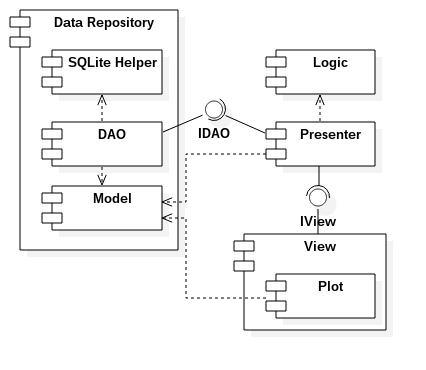
\includegraphics{uml_component}
	\caption{UML-діаграма компонентів}
	\label{fig:component}
\end{figure} 

Головними компонентами є:
\begin{itemize}
	\item \texttt{opencv} --- бібліотека функцій та алгоритмів комп'ютерного зору, обробки зображень і чисельних алгоритмів загального призначення з відкритим кодом;
	\item \texttt{keras} --- відкрита нейромережева бібліотека, написана мовою Python;
	\item \texttt{tensorflow} --- відкрита програмна бібліотека для машинного навчання цілій низці задач, розроблена компанією Google;
	\item \texttt{dlib} --- відкрита програмна бібліотека для машинного навчання;
	\item \texttt{gradients} --- реалізація методу середніх градієнтів;
	\item \texttt{main} --- головна компонента програми .
\end{itemize}

\subsubsection{Діаграма послідовності}
На рисунку~\ref{fig:sequence} зображена діаграма послідовності системи.

\begin{figure}[H]
	\centering
	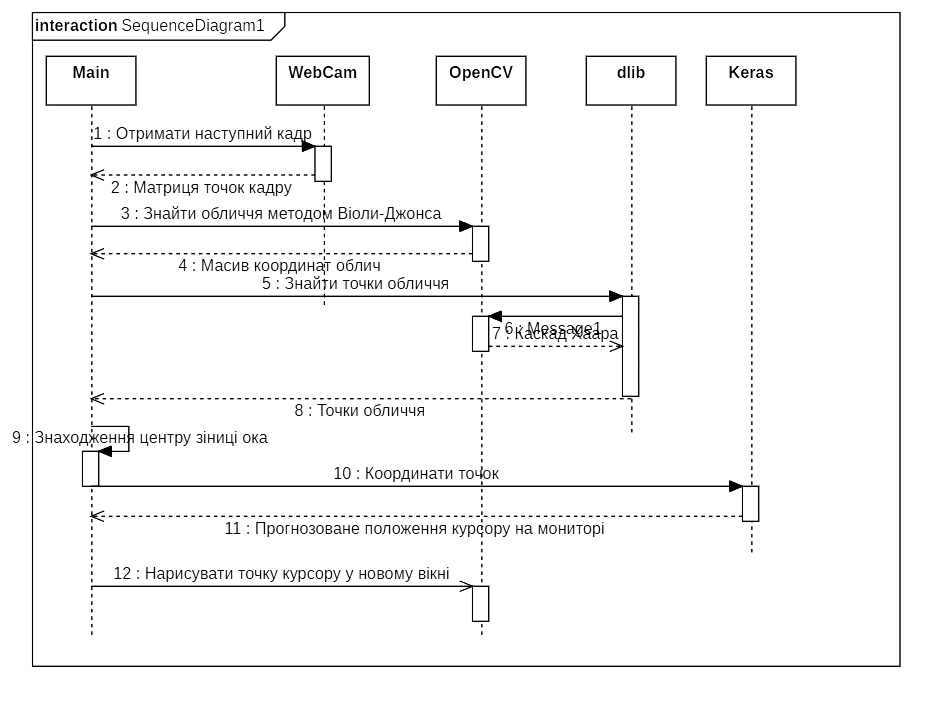
\includegraphics[width=\textwidth]{uml_sequence}
	\caption{UML-діаграма послідовності}
	\label{fig:sequence}
\end{figure} 

\subsubsection{Схема нейронної мережі}
На рисунку~\ref{fig:network} зображена схема нейронної мережі.

\begin{figure}[H]
	\centering
	\includegraphics[width=\textwidth]{network}
	\caption{Схема нейронної мережі}
	\label{fig:network}
\end{figure} 

Нейронна мережа буде складатися з п'яти шарів:
\begin{enumerate}[label={\arabic*-й ---}]
	\item має форму $256\times2$ та лінійну функцію активації; 
	\item має форму $128\times2$ та лінійну функцію активації; 
	\item має форму $64\times2$ та лінійну функцію активації; 
	\item має форму $256\times1$ та функцію активації сігмоїда; 
	\item має форму $2\times1$ та функцію активації сігмоїда. 
\end{enumerate}

На вхід подається матриця нормалізованих координат специфічних точок обличчя, які зображені на рисунку~\ref{fig:face}. 

\begin{figure}[H]
	\centering
	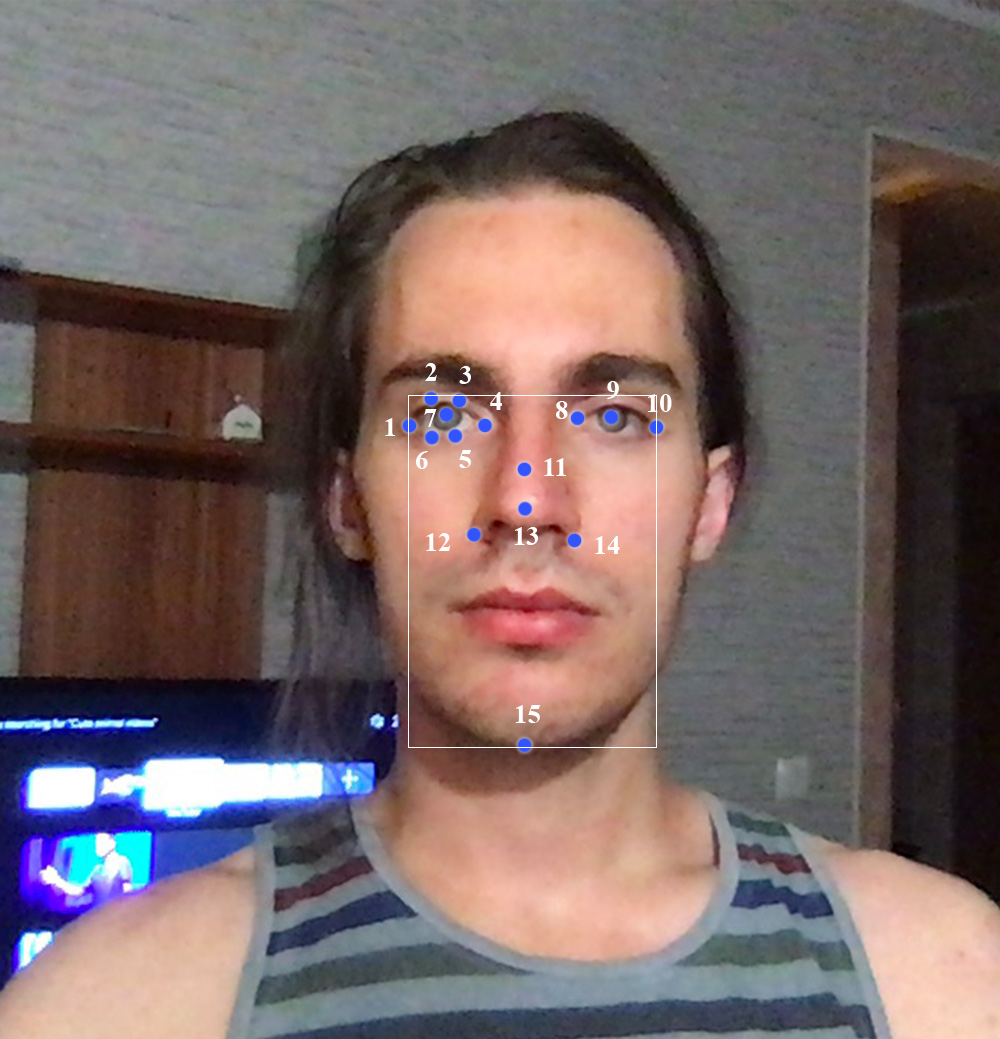
\includegraphics[width=0.6\textwidth]{face}
	\caption{Точки, які використовуються для визначення погляду}
	\label{fig:face}
\end{figure} 

\subsection{Обґрунтування вибору платформи розробки та інструментальних засобів}
\subsubsection{Мова програмування Python}
Python чудово підходить для вирішення задач машинного навчання, дозволяя писати стислий та експресивний код.

\subsubsection{Система управління версіями Git}
Використання системи контролю версії є необхідним для роботи над великими проектами.

Система контролю дозволяє зберігати попередні версії файлів та завантажувати їх за потребою. 
Вона зберігає повну інформацію про версію кожного з файлів, а також повну структуру проекту на всіх стадіях розробки.

Git --- розподілена система керування версіями файлів та спільної роботи. Git є однією з найефективніших, надійних і високопродуктивних систем керування версіями, що надає гнучкі засоби нелінійної розробки, що базуються на відгалуженні і злитті гілок.

\subsubsection{Середовище розробки застосунків Sublime Text 3}
Sublime Text 3 --- швидкий кросплатформенний редактор вихідних текстів програм. Підтримує плагіни, розроблені за допомогою мови програмування Python.

\section{Результати застосування розробленої системи}
\subsection{Стислі відомості щодо розгортання системи}

Вимоги до серверної машини наведено у таблиці~\ref{tab:sw_requirements}. 

\begin{table}[h]
	\caption{Мінімальні вимоги до серверного обладнання}
	\label{tab:sw_requirements}
	\begin{tabular}{l|l}
		Процесор & 1000 МГц \\ \hline
		ОЗП & 512 МБ \\ \hline
		Об'єм пам'яті диску & 64 ГБ 
	\end{tabular}
\end{table}

Програмне забезпечення серверу може бути встановлено на операційні системи родини \textit{Linux}, \textit{Windows} або \textit{macOS}.
Рекомендовано використовувати \acrshort{ssd} у якості накопичувача.

Для розгортання системи необхідно встановити наступні програми:
\begin{itemize}
	\item Apache Server v2.4.29+;
	\item SQLite v3.22.0+;
	\item PHP v7.2.2+;
\end{itemize}
та встановити драйвер взаємодії PHP з SQLite.

\subsection{Опис роботи з сайтом}
Робота з сайтом починається з процесу реєстрації користувача~(рисунок~\ref{fig:site_register}).
Незареєстрований користувач може переглядати товари та додавати їх до кошику, але не може оформити замовлення. 
\begin{figure}[H]
    \centering
    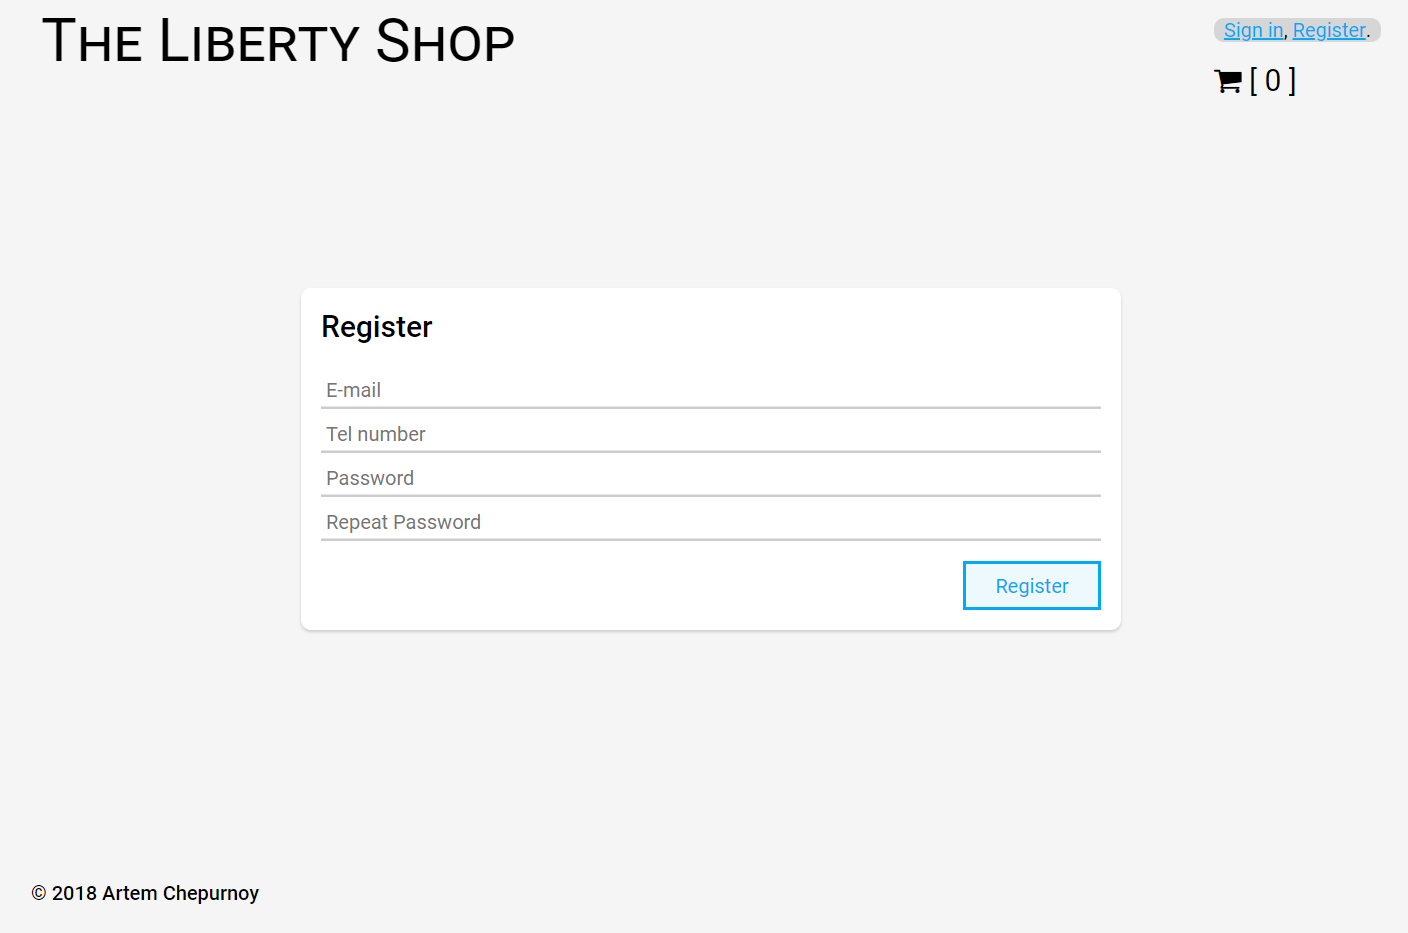
\includegraphics[width=0.8\textwidth]{screen_register}
    \caption{Сторінка реєстрації у системі}
    \label{fig:site_register}
\end{figure}

Після реєстрації користувач має увійти до системи~(рисунок~\ref{fig:site_login}).
\begin{figure}[H]
    \centering
    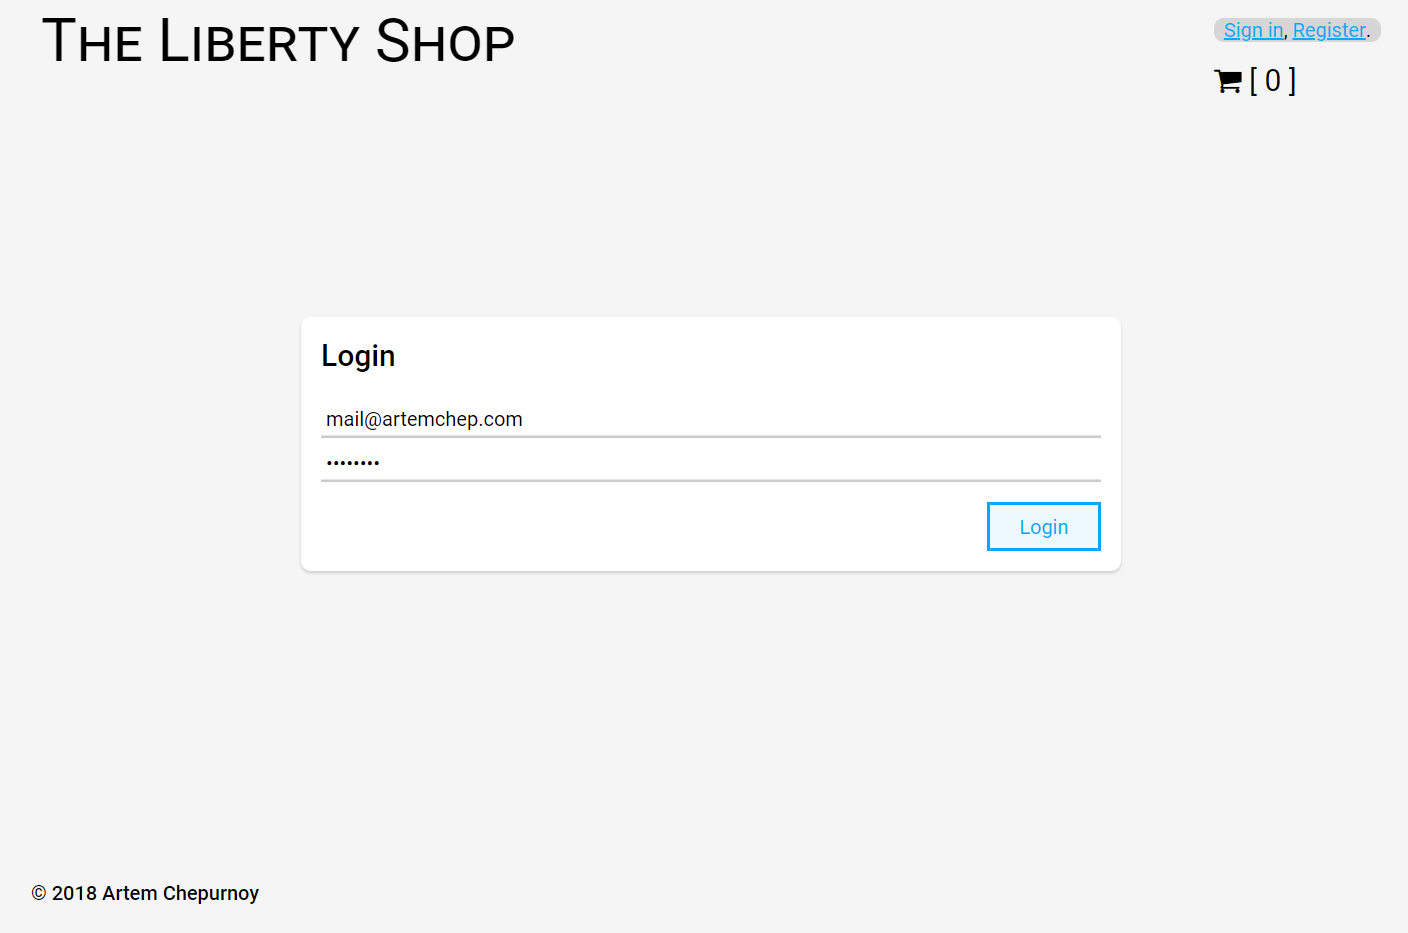
\includegraphics[width=0.8\textwidth]{screen_login}
    \caption{Сторінка входу до системи}
    \label{fig:site_login}
\end{figure}

Користувач може переглядати доступні товари на головній сторінці сайту.
Доступна можливість пошуку товару за ім'ям та категоріям.
\begin{figure}[H]
    \centering
    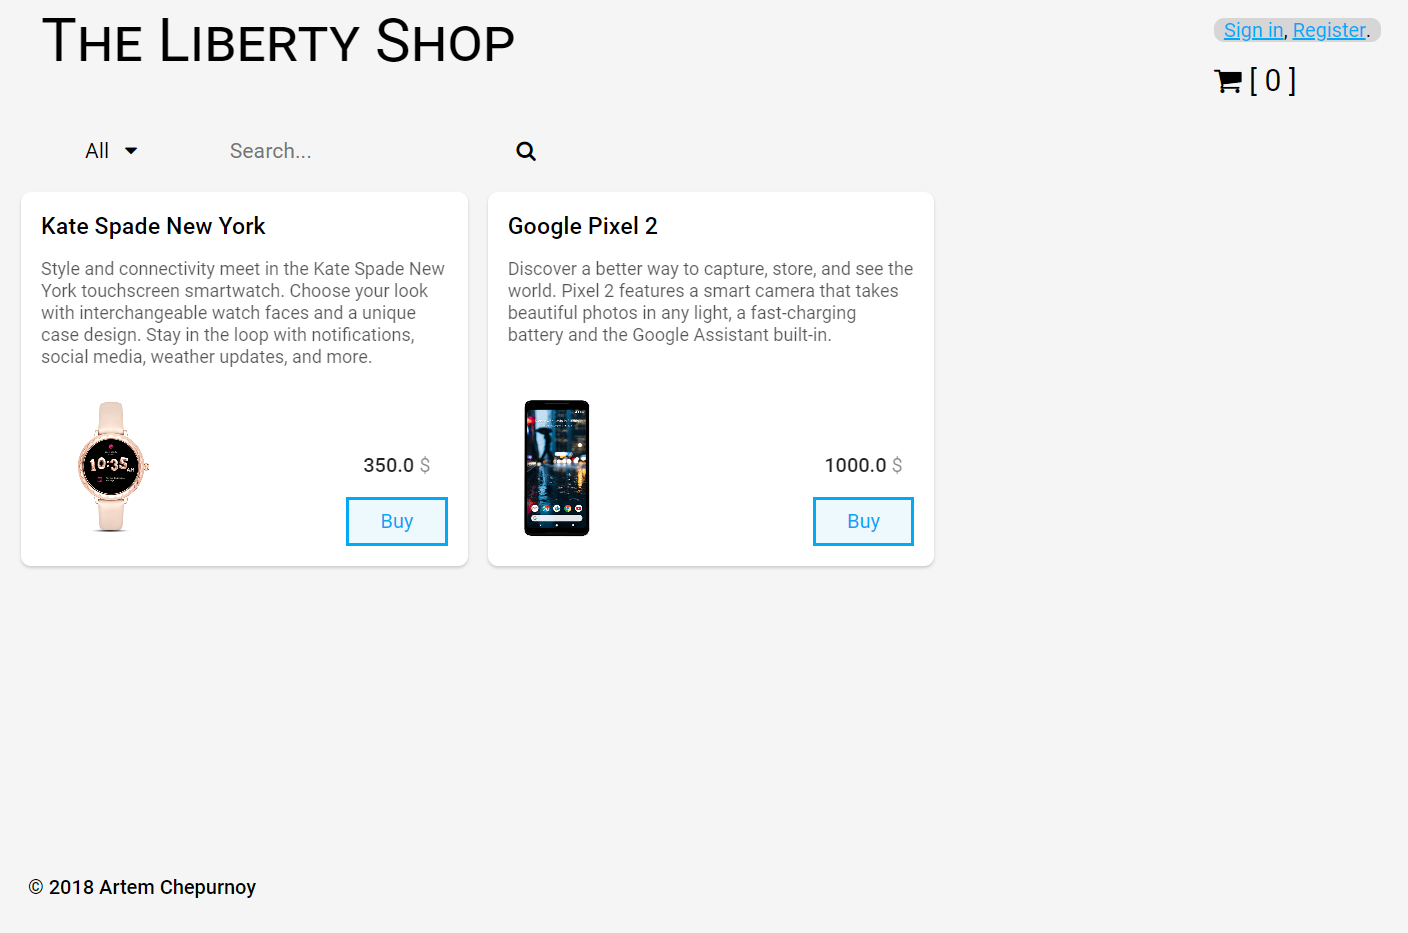
\includegraphics[width=0.8\textwidth]{screen_product__list}
    \caption{Головна сторінка ресурсу}
    \label{fig:site_product_list}
\end{figure}

Адміністратор та менеджери сайту мають на головній сторінці додаткові елементи~(рисунок~\ref{fig:site_product_list_admin}): 
\begin{itemize}
\item Кнопка редагування продуктів;
\item \textit{<<Add product>>} --- показати діалог додавання нового продукту;
\item \textit{<<Add category>>} --- показати діалог додавання нової категорії продуктів;
\item \textit{<<Edit category>>} --- показати діалог редагування та видалення категорії продуктів.
\end{itemize}
\begin{figure}[H]
    \centering
    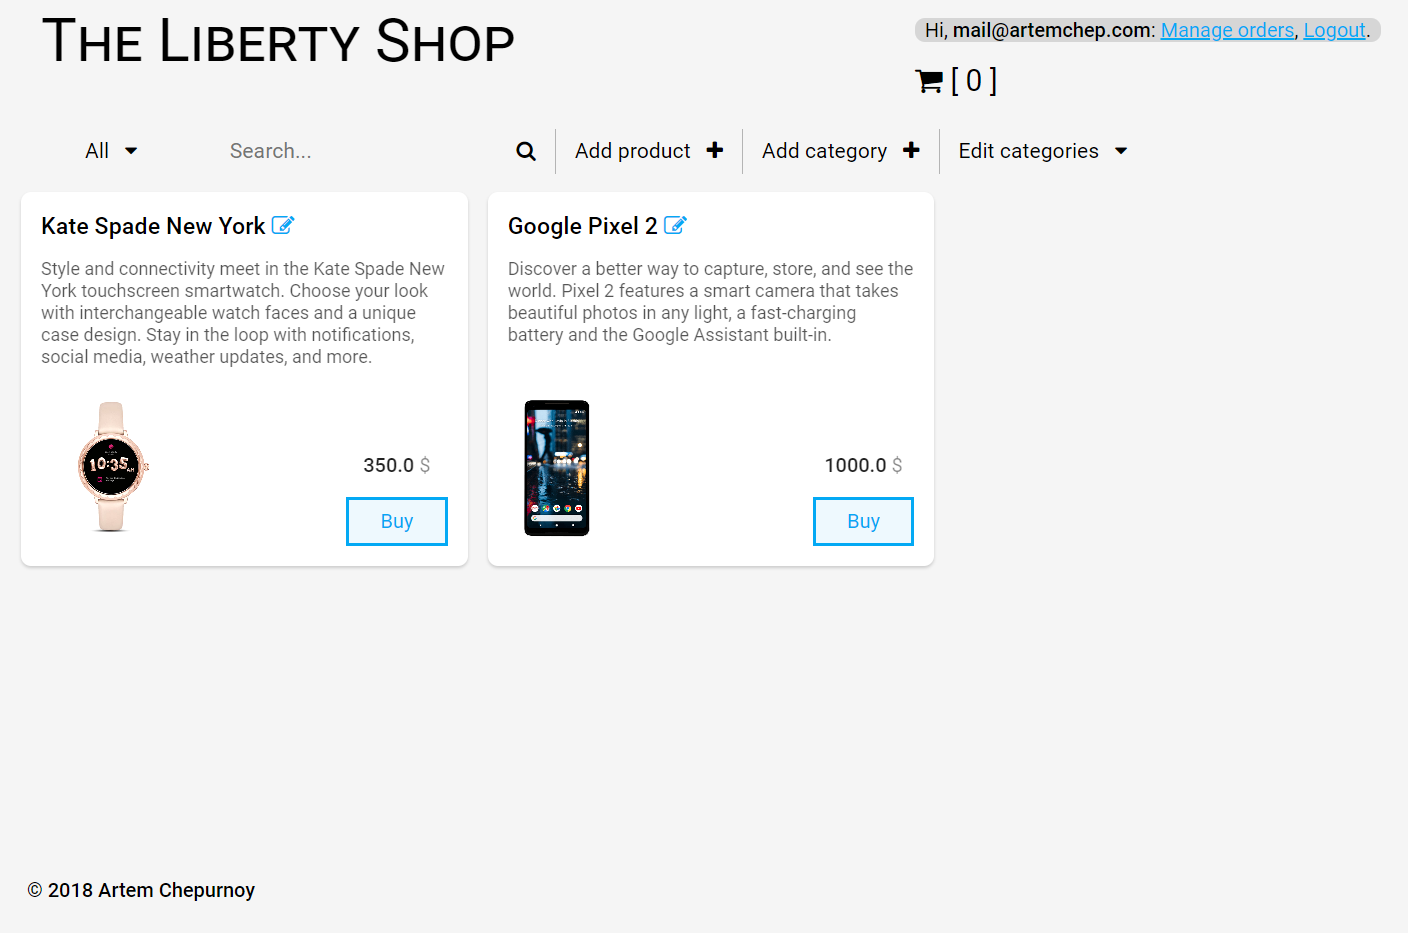
\includegraphics[width=0.8\textwidth]{screen_product__list__admin}
    \caption{Головна сторінка ресурсу (адміністратор)}
    \label{fig:site_product_list_admin}
\end{figure}

Діалог для створення нового продукту представлено на рисунку~\ref{fig:site_product_add}).

Продукт має такі властивості як категорія продуктів, назва, короткий опис, графічне зображення, ціна та розмірність.   
\begin{figure}[H]
    \centering
    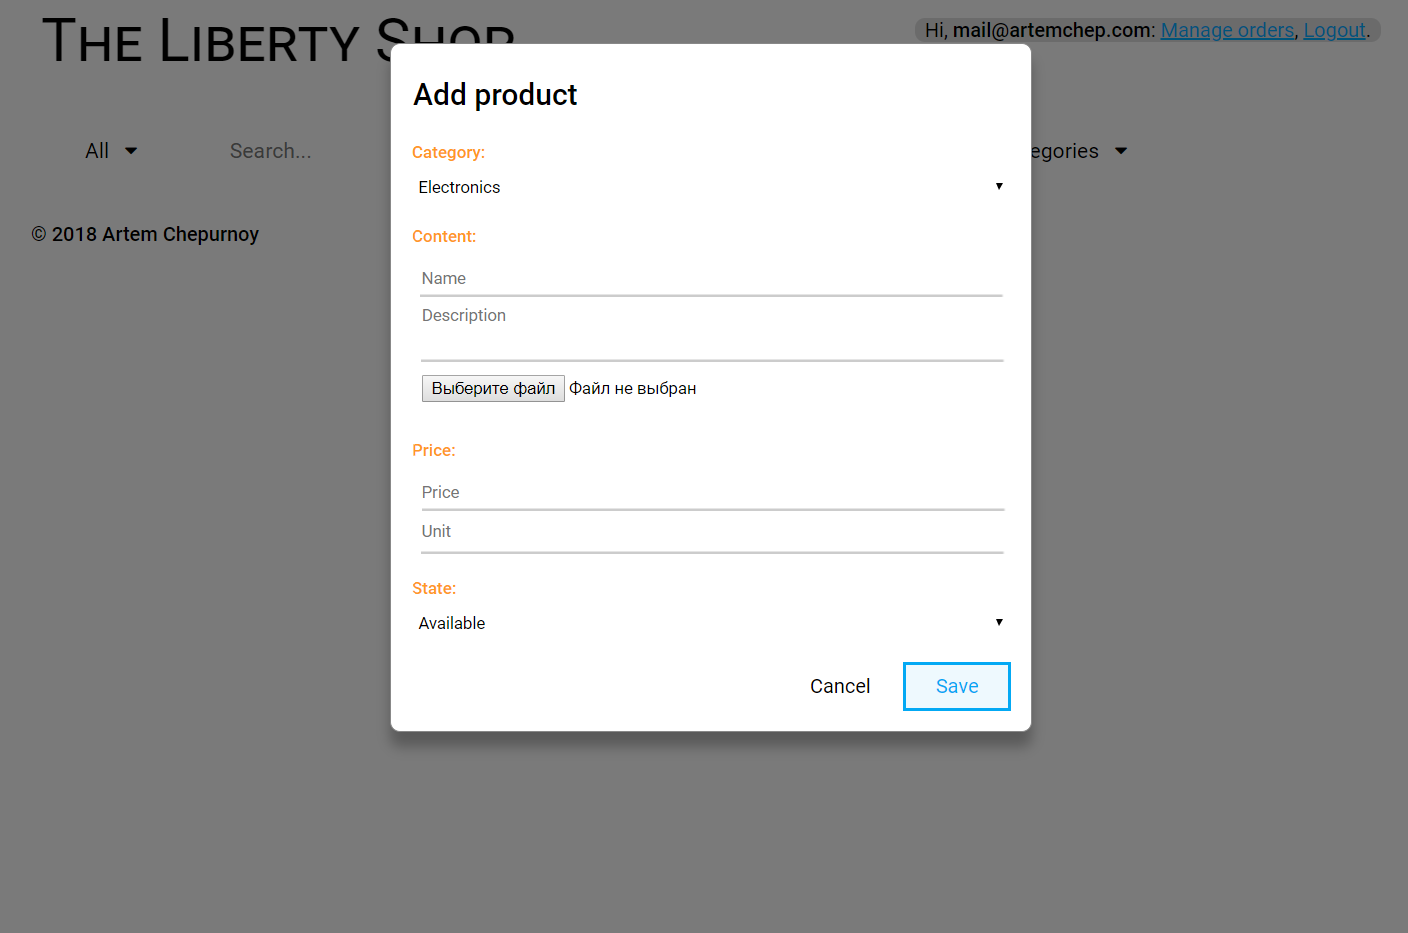
\includegraphics[width=0.8\textwidth]{screen_product_add}
    \caption{Діалог створення нового продукту}
    \label{fig:site_product_add}
\end{figure}

Адміністратор та менеджер ресурсу мають можливість переглянути список поточних або минулих замовлень~(рисунок~\ref{fig:site_order_list}), перемістити замовлення до архіву.
Є можливість фільтрування замовлень по даті створення, даті архівування, назві, категорії, кількості продуктів та ціні.   
\begin{figure}[H]
    \centering
    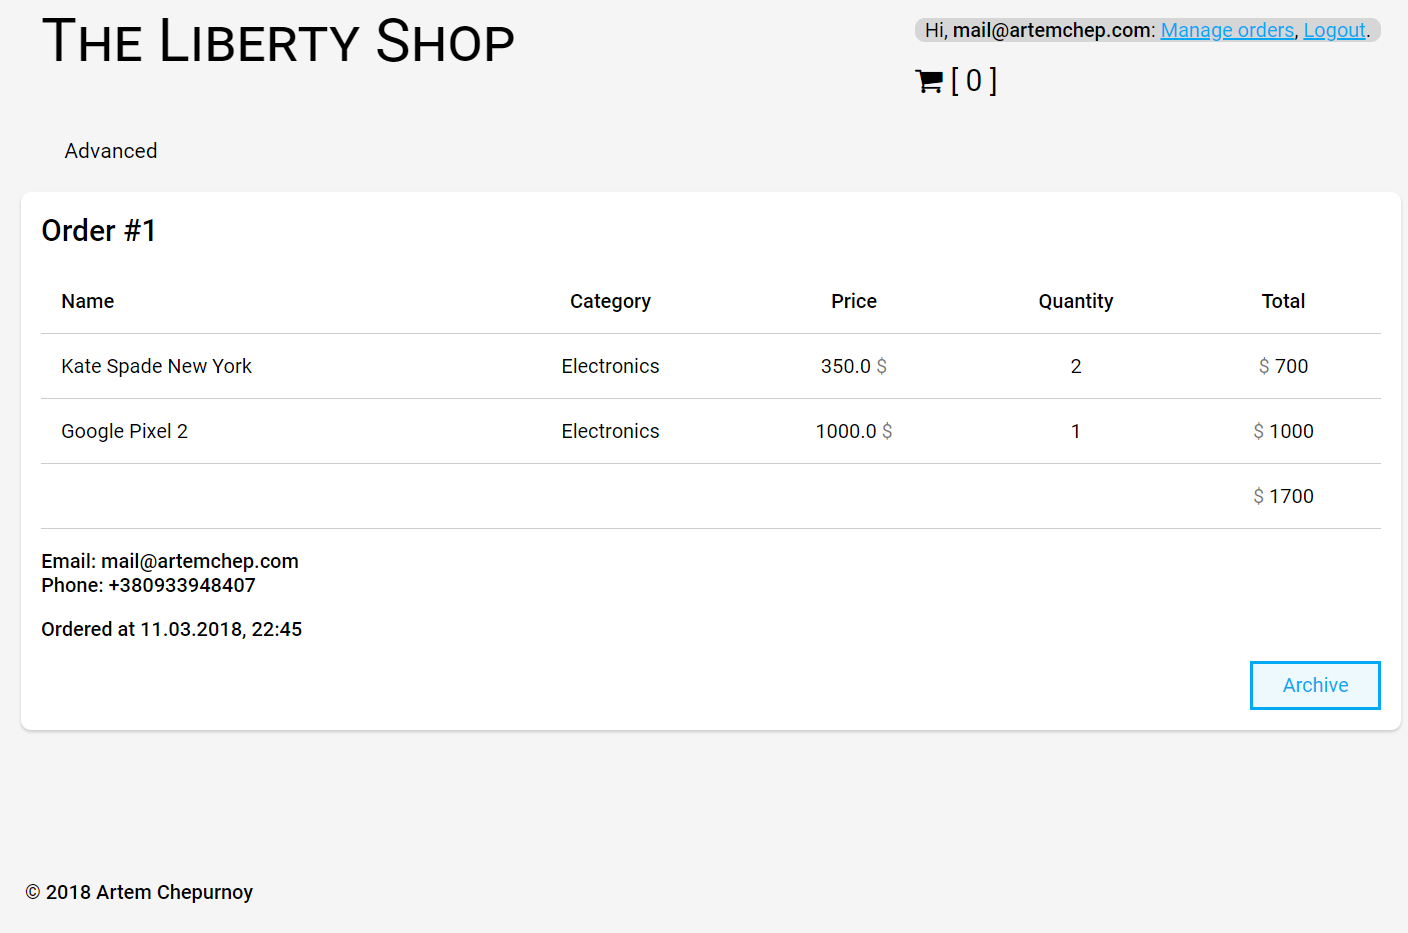
\includegraphics[width=0.8\textwidth]{screen_order__list}
    \caption{Сторінка керування замовленнями}
    \label{fig:site_order_list}
\end{figure}

\subsection{Результати тестування та рекомендації щодо удосконалення розробленої системи}
При тестуванні основною проблемою виявилася підтримка сайтом різних пристроїв та браузерів. 
При більш детальному вивченні стандартів HTML та CSS ця проблема була вирішена.

Одним із напрямків розвитку розробленої системи є співробітництво з іншими постачальниками, створення платформи для постачальників. 

% \section{Програмна реалізація системи}
\subsection{Особливості програмної реалізації системи, що розробляється}
Для розробки програмної системи була використані мова програмування Kotlin та застосовані патерни проектування типу GoF.

Були застосовані принципи SOLID~\cite{Arch2007}:
\begin{enumerate}
	\item Принцип єдиного обов'язку --- принцип об'єктно-орієнтованого програмування, який означає, що клас має бути створений для виконання лише однієї задачі, яку він повинен повністю інкапсулювати.
	      Отже, всі сервіси цього класу мають бути повністю підпорядковані її виконанню.
	      Результатом слідування цій концепції є наявність лише однієї причини для зміни класу.
	\item Принцип відкритості/закритості --- принцип об'єктно-орієнтованого програмування, який означає, що програмні сутності, такі як класи, модулі, функції, методи та ін. мають бути <<відкритими для розширення та закритими для змін>>.
	      Це означає, що вони можуть надавати можливість змінювати свою поведінку без або з мінімальними змінами коду.
	\item Принцип заміщення Лісков --- якщо $S$ підтип $T$, тоді об'єкти типу $T$ в програмі можуть бути заміщені об'єктами типу $S$ без будь-яких змін бажаних властивостей цієї програми.
	\item Принцип розділення інтерфейсів --- принцип схожий із принципом єдиного обов'язку.
	      Застосування даного принципу полягає у розділі занадто <<товстих>> інтерфейсів на менші та специфічні, щоб їх клієнти знали лише про ті методи, що необхідні для них у роботі.
	      Як результат, при зміні певного функціоналу, незмінними мають лишитися ті класи, що не використовують його.
	      Тобто виконання цього принципу допомагає системі залишатися гнучкою при внесенні до неї змін та лишатися простою для рефакторингу.
	\item Принцип інверсії залежностей.
	      Принцип формулюється наступним чином: модулі вищого рівня не повинні залежати від модулів нижчого рівня, обидва типи модулів повинні залежати від абстракцій; абстракції не повинні залежати від деталей реалізації, деталі реалізації повинні залежати від абстракцій.
\end{enumerate}

Система реалізована у парадігмі чистої архітектури, яка полягає в розділенні системи на 3 рівні~\cite{Arch2007}:
\begin{enumerate}
	\item Рівень даних --- рівень даних у чистому вигляді, що складається з сутностей, які є основними бізнес-правилами системи.
	\item Доменний рівень --- рівень бізнес-логіки додатку, що відповідає за основний функціонал системи, її поведінку та правила, що стосуються конкретного додатку.
	\item Рівень представлення --- рівень користувацького інтерфейсу, відображення даних, обробки користувацьких подій.
\end{enumerate}

\subsection{Тестування програмного забезпечення}
\subsubsection{Загальна теорія тестування}
Тестування --- перевірка відповідності реальної поведінки програми очікуваній, що здійснюється на кінцевому наборі тестів, який був обраний певним чином.
У більш широкому сенсі, тестування --- це одна з технік контролю якості, що включає в себе активності з планування робіт, проектування тестів, виконання тестування і аналізу отриманих результатів~\cite{Swebok}.

Верифікація --- це процес оцінки системи або її компонентів з метою визначення чи задовольняють результати поточного етапу розробки умовам, що були сформовані на початку цього етапу.
Тобто чи виконуються наші цілі, терміни, завдання по розробці проекту, визначені на початку поточної фази~\cite{Swebok}.

Валідація --- це визначення відповідності ПО, що розроблюється очікуванням і потребам користувача, вимогам до системи~\cite{Swebok}.

\subsubsection{Тестування програмної системи}
На першому етапі тестування необхідно провести модульне тестування усіх компонентів системи, які можуть бути протестовані окремо від інших у штучному середовищі тестування.
Для Unit-тестування використовується засоб автоматизації тестування Kotest.

Такий вибір зумовлений простотою інтеграції з Kotlin.
Kotest надає великий об'єм валідаційних методів, завдяки яким можна легко та ефективно тестувати як модулі обробки даних та взаємодії з базами даних, так і модулі вводу та виводу інформації~\cite{Kotest}.

Фрагмент застосованих Kotest тестів для валідації коректної роботи класу \texttt{GlobeHipster} приведено нижче:
\lstinputlisting{code/tests.kt}

\subsection{Інтерфейс програмного забезпечення}
Розроблена програмна система має консольний інтерфейс. Для запуску моделювання необхідно виконати такі команди:
\begin{lstlisting}
> jar kagent.jar --period=14 --time=5 configuration_a.json configuration_b.json
\end{lstlisting}
\begin{description}
	\item[де] \texttt{kagent.jar} --- назва бінарного файла програмної системи;
	\item \texttt{--period=14} --- період поповнення запасів регіональними та національними складами, у днях;
	\item \texttt{--time=5} --- час моделювання системи, у секундах;
	\item \texttt{configuration\_a.json} --- шлях до файлу конфігурації першого варіанта логістичної системи;
	\item \texttt{configuration\_b.json} --- шлях до файлу конфігурації другого варіанта логістичної системи.
\end{description}

В процесі моделювання логістичної системи у консоль виводиться поточний стан логістичної системи.
Фрагмент логування початкової загрузки конфігурації логістичної системи:
\begin{lstlisting}
Connecting Киев to Пирятин by 154.0 km. road
Connecting Житомир to Винница by 127.0 km. road
Connecting Николаев to Мелитополь by 299.0 km. road
Connecting Николаев to Саки by 325.0 km. road
Connecting Днепропетровск to Днепродзержинск by 45.0 km. road
Connecting Львов to Дубляны by 9.0 km. road
\end{lstlisting}

Фрагмент логування процесу моделювання логістичної системи:
\begin{lstlisting}
[432]
.     Current time is 432 days.
.    service level is 87%.
. avg. stock level is 92%.
[433]
.     Current time is 433 days.
.    service level is 88%.
. avg. stock level is 92%.
[434]
.     Current time is 434 days.
.    service level is 88%.
. avg. stock level is 91%.
\end{lstlisting}

Для генерації дампу поточного стану системи у файл необхідно натиснути клавішу <<S>> під час процесу моделювання, для призупинення виконування програми необхідно натиснути клавішу <<P>>.
Графічний інтерфейс складається з двох частин: меню та панелі поточного стану моделі.

Після закінчення часу на моделювання системи показується окно з динамікою зміни рівня сервісу за час моделювання (рисунок~\ref{fig:graph_sample}).

\begin{figure}[H]
	\centering
	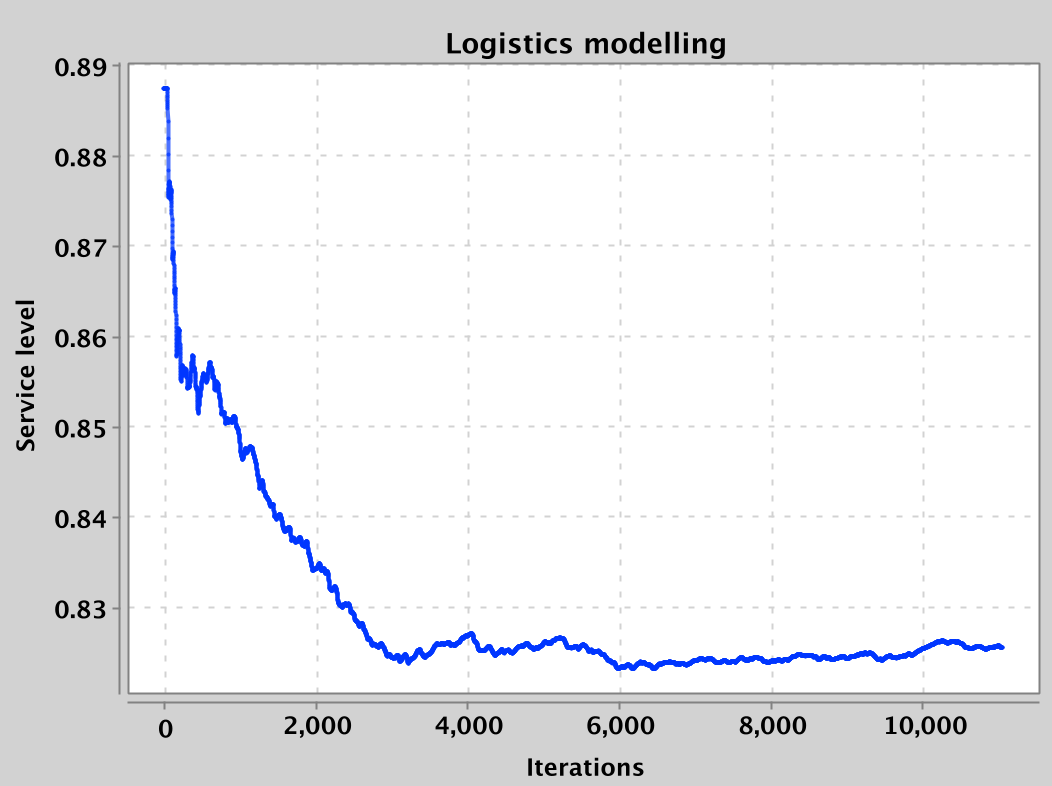
\includegraphics[width=0.6\textwidth]{graph_sample}
	\caption{Динаміка зміни рівня сервісу}
	\label{fig:graph_sample}
\end{figure}

\subsection{Аналіз продуктивності програмного забезпечення}
Розроблений програмний продукт широко використовує паралельні обчислення. 
В якості основи для паралельних обчислень було використано технологію Kotlin coroutines.

Для порівняння роботи програми у багатопотоковому режимі та однопотоковому режимі був проведений експеримент: моделювання логістичної системи~\cite{Годлевський2019} з обмеженої кількістю агентів на регіональному шару. Результат експерименту представлено на рисунку~\ref{fig:performance}.

\begin{figure}[H]
	\centering
	\begin{tikzpicture}
		\begin{axis}[
				scaled y ticks = false,
				xlabel={Кількість кінцевих споживачів продукції},
				xlabel near ticks,
				ylabel={Ітерацій за 100 мілісекунд},
				ylabel near ticks,
				ymajorgrids=true,
				line width=0.4mm,
				grid style=dashed,
			]
			\addplot table [x=n, y=i] {data/test_cpu.csv};
			\addplot table [x=n, y=z] {data/test_cpu.csv};
			\legend{багатопотоковий режим,однопотоковий режим}
		\end{axis}
	\end{tikzpicture}
	\caption{Результати оцінки продуктивності~\acrshort{sw}}
	\label{fig:performance}
\end{figure}

Програмний продукт у багатопотоковому режимі працює в $\~5$ разів швидше ніж у однопотоковому режимі. 
Це обумовлено тим що експеримент проводився на комп'ютері з чотирма ядрами процессору і у многопоточному режимі програма використовує всі ресурси всіх процесорів, а в однопотоковому режимі тільки один.  

\subsection{Аналіз результатів дослідження}
Початкова конфігурація була взята з роботи~\cite{Годлевський2019} яка в свою чергу базується на роботі <<Моделі і інформаційна технологія стратегічного управління логістичною системою дистрибуції>>~\cite{Stankevich}.

З метою формування множини ефективних рішень конфігурації логістичної системи в роботі були приведені прорахунки для двох варіантів базового рівня сервісу на регіональних складах: $84.13\%$, $97.72\%$. Для кожного базового рівня сервісу розглядалися тривалості циклів замовлень з виробничого на національний і далі на регіональний рівні: 2, 3 і 4 тижні.

Таким чином було сформовано 36 конфігурацій логістичних мереж, для кожної з котрих було проведено моделювання рівня сервісу.

Результати експерименту приведені в таблиці~\ref{tab:results}.

{
\small
\tabulinesep=1.2mm
\begin{longtabu} to \textwidth {|X[1,c]|X[1,c]|X[1,c]|X[1,c]|X[1,c]|}
	\caption{Результати експерименту моделювання конфігурацій логістичних систем}
	\label{tab:results} \\
	\hline
	Кількість регіональних складів & Тривалість циклу, тижнів & Базовий рівень страхового запасу, \% & Сумарні логістичні витрати~\cite{Годлевський2019} & Мережевий рівень сервісу \\
	\hline
	\endfirsthead
	\caption*{Закінчення таблиці \thetable{}}\\
	\hline
	Кількість регіональних складів & Тривалість циклу, тижнів & Базовий рівень страхового запасу, \% & Сумарні логістичні витрати~\cite{Годлевський2019} & Мережевий рівень сервісу \\
	\hline
	\endhead
	5 & \multirow{4}{*}{2} & \multirow{12}{*}{$84.13$} & $183729.3882$ & $0.864868$ \\ \cline{1-1}\cline{4-5}
	6 & & & $185253.5535$ & $0.868993$ \\ \cline{1-1}\cline{4-5}
	7 & & & $185649.9391$ & $0.871659$ \\ \cline{1-1}\cline{4-5}
	8 & & & $185935.0956$ & $0.873573$ \\ \cline{1-2}\cline{4-5}

	5 & \multirow{4}{*}{3} & & $195332.5978$ & $0.830533$ \\ \cline{1-1}\cline{4-5}
	6 & & & $196856.7631$ & $0.831683$ \\ \cline{1-1}\cline{4-5}
	7 & & & $197253.1487$ & $0.831786$ \\ \cline{1-1}\cline{4-5}
	8 & & & $197538.3052$ & $97$ \\ \cline{1-2}\cline{4-5}

	5 & \multirow{4}{*}{4} & & $206935.8074$ & $0.793313$ \\ \cline{1-1}\cline{4-5}
	6 & & & $208459.9727$ & $0.800558$ \\ \cline{1-1}\cline{4-5}
	7 & & & $208856.3583$ & $0.804958$ \\ \cline{1-1}\cline{4-5}
	8 & & & $209141.5148$ & $0.808666$ \\ \hline

	5 & \multirow{4}{*}{2} & \multirow{12}{*}{$97.72$} & $187478.0538$ & $0.931035$ \\ \cline{1-1}\cline{4-5}
	6 & & & $189002.2191$ & $0.938148$ \\ \cline{1-1}\cline{4-5}
	7 & & & $189398.6047$ & $0.939289$ \\ \cline{1-1}\cline{4-5}
	8 & & & $189683.7612$ & $0.940954$ \\ \cline{1-2}\cline{4-5}

	5 & \multirow{4}{*}{3} & & $200955.5962$ & $0.895327$ \\ \cline{1-1}\cline{4-5}
	6 & & & $202479.7615$ & $0.896253$ \\ \cline{1-1}\cline{4-5}
	7 & & & $202876.1471$ & $0.898870$ \\ \cline{1-1}\cline{4-5}
	8 & & & $203161.3036$ & $0.900588$ \\ \cline{1-2}\cline{4-5}

	5 & \multirow{4}{*}{4} & & $214433.1386$ & $0.859070$ \\ \cline{1-1}\cline{4-5}
	6 & & & $215957.3039$ & $0.867487$ \\ \cline{1-1}\cline{4-5}
	7 & & & $216353.6895$ & $0.870390$ \\ \cline{1-1}\cline{4-5}
	8 & & & $216638.846$ & $0.877827$ \\ \hline
\end{longtabu}
}

Візуалізація зміни рівня сервісу представлені на рисунках~\ref{fig:graph_84},~\ref{fig:graph_99}.

\begin{figure}[H]
	% \def\axisdefaultwidth{14cm}
	% \def\axisdefaultheight{10сm}
	\centering
	\begin{tikzpicture}
		\begin{axis}[
				legend style={font=\footnotesize,at={(1.6,1.0)},anchor=north east},
				xmin=0,
				xmax=10000,
				xlabel={Номер ітерації моделювання},
				xlabel style={yshift=-1cm},
				ylabel={Рівень сервісу},
				ylabel near ticks,
				ymajorgrids=true,
				grid style=dashed,
				line width=0.4mm,
				mark size=0pt,
				mark = none,
				smooth
			]
			\addplot table [x=i, y=1] {data/dynamic_84.csv};
			\addplot table [x=i, y=2] {data/dynamic_84.csv};
			\addplot table [x=i, y=3] {data/dynamic_84.csv};
			\addplot table [x=i, y=4] {data/dynamic_84.csv};
			\addplot table [x=i, y=5] {data/dynamic_84.csv};
			\addplot table [x=i, y=6] {data/dynamic_84.csv};
			\addplot table [x=i, y=7] {data/dynamic_84.csv};
			\addplot table [x=i, y=8] {data/dynamic_84.csv};
			\addplot table [x=i, y=9] {data/dynamic_84.csv};
			\addplot table [x=i, y=10] {data/dynamic_84.csv};
			\addplot table [x=i, y=11] {data/dynamic_84.csv};
			\addplot table [x=i, y=12] {data/dynamic_84.csv};
			\legend{5 складів; 2 тижня,6 складів; 2 тижня,7 складів; 2 тижня,8 складів; 2 тижня,5 складів; 3 тижня,6 складів; 3 тижня,7 складів; 3 тижня,8 складів; 3 тижня,5 складів; 4 тижня,6 складів; 4 тижня,7 складів; 4 тижня,8 складів; 4 тижня}
		\end{axis}
	\end{tikzpicture}
	% 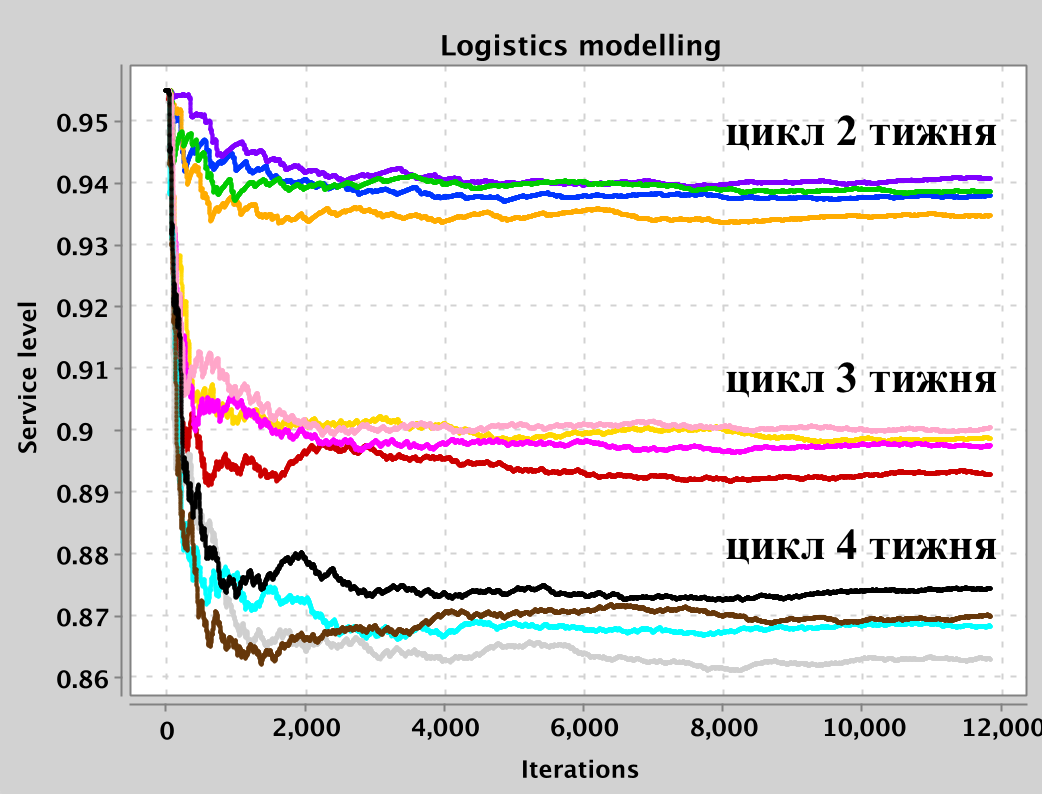
\includegraphics[width=0.6\textwidth]{graph_99}
	\caption{Динаміка зміни рівня сервісу для групи конфігурацій з базовим рівнем страхового запасу рівним $84.13$}
	\label{fig:graph_84}
\end{figure}

\begin{figure}[H]
	% \def\axisdefaultwidth{14cm}
	% \def\axisdefaultheight{10сm}
	\centering
	\begin{tikzpicture}
		\begin{axis}[
				legend style={font=\footnotesize,at={(1.6,1.0)},anchor=north east},
				xmin=0,
				xmax=10000,
				xlabel={Номер ітерації моделювання},
				xlabel style={yshift=-1cm},
				ylabel={Рівень сервісу},
				ylabel near ticks,
				ymajorgrids=true,
				grid style=dashed,
				line width=0.4mm,
				mark size=0pt,
				mark = none,
				smooth
			]
			\addplot table [x=i, y=1] {data/dynamic_97.csv};
			\addplot table [x=i, y=2] {data/dynamic_97.csv};
			\addplot table [x=i, y=3] {data/dynamic_97.csv};
			\addplot table [x=i, y=4] {data/dynamic_97.csv};
			\addplot table [x=i, y=5] {data/dynamic_97.csv};
			\addplot table [x=i, y=6] {data/dynamic_97.csv};
			\addplot table [x=i, y=7] {data/dynamic_97.csv};
			\addplot table [x=i, y=8] {data/dynamic_97.csv};
			\addplot table [x=i, y=9] {data/dynamic_97.csv};
			\addplot table [x=i, y=10] {data/dynamic_97.csv};
			\addplot table [x=i, y=11] {data/dynamic_97.csv};
			\addplot table [x=i, y=12] {data/dynamic_97.csv};
			\legend{5 складів; 2 тижня,6 складів; 2 тижня,7 складів; 2 тижня,8 складів; 2 тижня,5 складів; 3 тижня,6 складів; 3 тижня,7 складів; 3 тижня,8 складів; 3 тижня,5 складів; 4 тижня,6 складів; 4 тижня,7 складів; 4 тижня,8 складів; 4 тижня}
		\end{axis}
	\end{tikzpicture}
	% 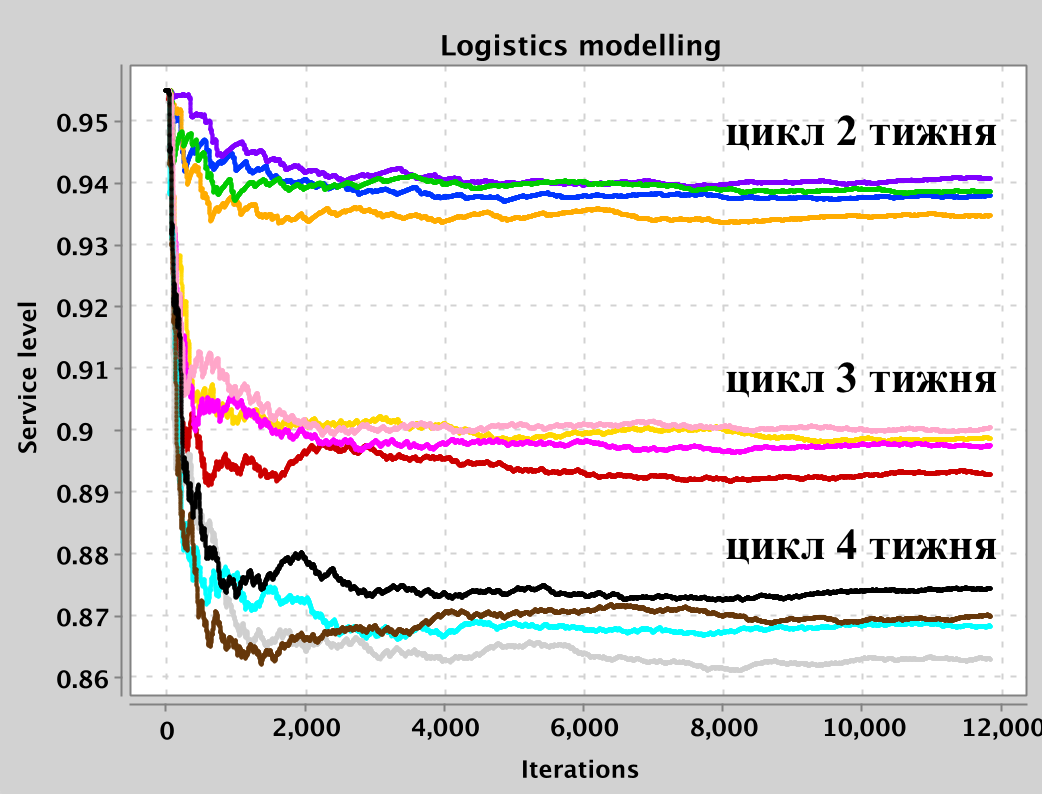
\includegraphics[width=0.6\textwidth]{graph_99}
	\caption{Динаміка зміни рівня сервісу для групи конфігурацій з базовим рівнем страхового запасу рівним $97.72$}
	\label{fig:graph_99}
\end{figure}

Наглядна графічна інтерпретація результатів з таблиці~\ref{tab:results} зображена на рисунку~\ref{fig:results}.

\begin{figure}[H]
	\centering
	\begin{tikzpicture}
		\begin{axis}[
				scaled y ticks = false,
				xlabel={Сумарні логістичні витрати},
				xlabel style={yshift=-1cm},
				ylabel={Мережевий рівень сервісу},
				ylabel near ticks,
				enlargelimits=false,
				line width=0.4mm,
				ymajorgrids=true,
				grid style=dashed,
			]
			\addplot+[
				only marks,
				scatter,
				mark=halfcircle*,
				mark size=2.9pt]
			table[meta=y]
				{data/results.csv};
		\end{axis}
	\end{tikzpicture}
	\caption{Результати експерименту моделювання конфігурацій логістичних систем}
	\label{fig:results}
\end{figure}

Проведемо аналіз отриманих результатів.
Незалежно від тривалості циклів замовлень рівень сервісу збільшується зі збільшенням кількості регіональних складів.
Це можна пояснити тим, що збільшується загальний розмір страхових запасів.
Мережевий рівень сервісу зменшується зі збільшенням тривалості циклів замовлень. Це пов'язано з тим, що при меншому циклі замовлень є більше можливостей на адаптацію до змін попиту.
Зі збільшенням базового рівня сервісу збільшується рівень мережевого сервісу.
Виходячи з проведеного аналізу, можна зробити висновок, що безліч ефективних рішень знаходиться в лівому верхньому кутку графіка (рис.~\ref{fig:results}). Залежно від пріоритету експерту по відношенню до критеріїв: сумарні логістичні витрати, мережевий рівень сервісу вибирається прийнятна конфігурація логістичної системи.

Подальше використання отриманих результатів пов'язане з визначенням стійкості рівня сервісу до різноманітних надзвичайних ситуацій. Отримані результати є основою для формування організаційної структури управління логістичною системою дистрибуції.

% \section{Техніко-економічне обґрунтування проекту}
Мета даного розділу --- провести розрахунок сукупної величини витрат, пов'язаних з розробкою програмної компоненти для аналізу стійкості функціонування логістичних систем.

Витрати на розробку будуть проводитись за наступними пунктами:
\begin{itemize}
	\item витрат на апаратне забезпечення;
	\item витрат на програмне забезпечення;
	\item витрат на зовнішні постачальники послуг;
	\item витрат на оплату праці.
\end{itemize}

Для розробки програмних компонентів агентної платформи використовується мова програмування Kotlin.
Проект потребує спеціалістів які володіють зазначеною мовою на рівні не нижче середнього на ринку, через високу складність конструювання програмного забезпечення.
Даний проект розробляється командою з трьох програмних інженерів зазначеної спеціалізації, проектного менеджера, експерта з логістичних систем та тестувальника.
Термін розробки складає два року.

В якості методології розробки буде використана методологія XP.

\subsection{Апаратне забезпечення}
Для команди розробників необхідні апаратні компоненти які задовольняють таким вимогам:
\begin{itemize}
	\item процесор: Intel core i7 5 покоління;
	\item оперативна пам'ять: DDR4 16 GB;
	\item внутрішня пам'ять: SSD 256 GB.
\end{itemize}

Оптимальною конфігурацією для роботи буде ноутбук MacBook Pro 2015 року з 16 ГБ оперативної пам'яті.

Для проектного менеджера необхідні апаратні компоненти які задовольняють таким вимогам:
\begin{itemize}
	\item процесор: Intel core i3 5 покоління;
	\item оперативна пам'ять: DDR4 4 ГБ;
	\item внутрішня пам'ять: SSD 256 ГБ.
\end{itemize}

Оптимальною конфігурацією для роботи буде ноутбук MacBook Air 2015 року з 4 ГБ оперативної пам'яті.

Для експерта з логістичних систем та тестувальника необхідні апаратні компоненти які задовольняють таким вимогам:
\begin{itemize}
	\item процесор: Intel core i7 5 покоління;
	\item оперативна пам'ять: DDR4 8 ГБ;
	\item внутрішня пам'ять: SSD 256 ГБ.
\end{itemize}

Оптимальною конфігурацією для роботи буде ноутбук MacBook 2015 року з 8 ГБ оперативної пам'яті.

Вартість кожної апаратної компоненти представлена в таблиці~\ref{tab:economy_hardware}.

{
\tabulinesep=1.2mm
\begin{longtabu} to \textwidth {|X[3,l]|X[1,c]|}
	\caption{Вартість апаратних компонентів необхідних для команди}
	\label{tab:economy_hardware} \\
	\hline
	Модель ноутбука & Вартість, грн. \\
	\hline
	\endfirsthead
	\caption*{Закінчення таблиці \thetable{}}\\
	\hline
	Модель ноутбука & Вартість, грн. \\
	\hline
	\endhead

	MacBook Pro 15 2015 Retina Z0W60002T & $35499$~\cite{MacBookProPrice} \\ \hline
	MacBook Pro 15 2015 Retina Z0W70001U & $43299$~\cite{MacBookProPrice} \\ \hline
	MacBook Air 2015 Z0X5000BR & $29999$~\cite{MacBookAirPrice} \\ \hline
\end{longtabu}
}

Вартість апаратного забезпечення для команди розробників:
\[
	C_{hw:dev} = 43299 \cdot 3 = 129897 \textup{ грн.}
\]
, для проектного менеджера:
\[
	C_{hw:pm} = 29999 = 29999 \textup{ грн.}
\]
, для експерта з логістичних систем:
\[
	C_{hw:expert} = 35499 = 35499 \textup{ грн.}
\]
, для тестувальника:
\[
	C_{hw:test} = 35499 = 35499 \textup{ грн.}
\]

Загальна вартість апаратних компонентів необхідних для проектної команди дорівнює:
\begin{gather*}
	C_{hw} = C_{hw:dev} + C_{hw:pm} + C_{hw:expert} + C_{hw:dev} = \\
	= 129897 + 29999 + 35499 + 35499 = \\
	= 230894 \textup{ грн.}
\end{gather*}

\subsection{Витрати на оплату праці}
Вартість роботи проектної команди зображена в таблицях~\ref{tab:economy_hr_1},~\ref{tab:economy_hr_2}.

	{
		\tabulinesep=1.2mm
		\begin{longtabu} to \textwidth {|X[4,l]|X[1,l]|X[3,l]|}
			\caption{Розподіл заробітної плати проектної команди}
			\label{tab:economy_hr_1} \\
			\hline
			Учасник проекту & Посада & Заробітна плата, дол. / год. \\
			\hline
			\endfirsthead
			\caption*{Закінчення таблиці \thetable{}}\\
			\hline
			Учасник проекту & Посада & Заробітна плата, дол. / год. \\
			\hline
			\endhead

			Менеджер проекту & Middle & $8.25$~\cite{SalaryProgrammer} \\ \hline
			Kotlin розробник №1 & Senior & $15.5$~\cite{SalaryProgrammer} \\ \hline
			Kotlin розробник №2 & Middle & $9$~\cite{SalaryProgrammer} \\ \hline
			Kotlin розробник №3 & Middle & $9$~\cite{SalaryProgrammer} \\ \hline
			Експерт в логістичних системах & Middle & $11$~\cite{SalaryLogisticExpert} \\ \hline
			QA інженер & Middle & $6$~\cite{SalaryProgrammer} \\ \hline
		\end{longtabu}
	}
	{
		\small
		\tabulinesep=1.2mm
		\begin{longtabu} to \textwidth {|X[2,l]|X[1,l]|X[1,l]|X[1,l]|X[1,l]|X[1,l]|X[1,l]|}
			\caption{Розподіл робочих годин та вартості роботи проектної команди}
			\label{tab:economy_hr_2} \\
			\hline
			Фаза проекту & Менеджер проекту, год. & Kotlin розробник №1, год. & Kotlin розробник №2, год. & Kotlin розробник №3, год. & Експерт в логістичних системах, год. & QA інженер, год. \\
			\hline
			\endfirsthead
			\caption*{Закінчення таблиці \thetable{}}\\
			\hline
			Фаза проекту & Менеджер проекту, год. & Kotlin розробник №1, год. & Kotlin розробник №2, год. & Kotlin розробник №3, год. & Експерт в логістичних системах, год. & QA інженер, год. \\
			\hline
			\endhead

			Початкова фаза (1-6 місяць) & 200 & 100 & 0 & 0 & 100 & 0 \\ \hline
			Фаза уточнення (7-9 місяць) & 200 & 200 & 50 & 50 & 200 & 50 \\ \hline
			Фаза конструювання (10-15 місяць) & 100 & 200 & 200 & 200 & 50 & 200 \\ \hline
			Фаза впровадження (10-15 місяць) & 100 & 100 & 150 & 150 & 50 & 200 \\ \hline
			$\sum$ & 600 & 600 & 400 & 400 & 400 & 450 \\ \hline
		\end{longtabu}
	}

Загальна вартість роботи проектної команди:
\begin{gather*}
	C_{hr} = \\ = 600 \cdot 8.25 + 600 \cdot 15.5 + 400 \cdot 9 + 400 \cdot 9 + 400 \cdot 11 + 450 \cdot 6 = \\ = 28550 \textup{ дол.}
\end{gather*}

Згідно із курсом долара~\cite{Dollar} (станом на 20.04.20) вартість на команду розробки у гривнях становить:
\begin{gather*}
	C_{hr} = 28550 \cdot 27.2 = 776560 \textup{ грн.}
\end{gather*}

\subsection{Витрати на програмне забезпечення}
На усіх компьютерах команди буде встановлена безкоштовна операційна система mac OS. Серед основних цілей mac os -- надання сучасного й водночас стабільного програмного забезпечення для пересічного користувача із сильним акцентом на простоту встановлення та користування~\cite{MacOS}.

Розробка програмних компонентів агентної платформи буде виконуватись із використання середовища для розробки Intellij Idea Ultimate Edition. Згідно із курсом долара~\cite{Dollar} (станом на 20.04.20) вартість на використання середовища у гривнях становить~\cite{IDEA}:
\[
	C_{sw:idea} = 449 \cdot 1.5 \cdot 3 \cdot 27.2 = 54957.6 \textup{ грн.}
\]

Для забезпечення приватності, версіонування та збереження коду, та тестування системи буде використана система контролю версій Git, а саме холдінг GitHub. Згідно із курсом долара~\cite{Dollar} (станом на 20.04.20) вартість на використання сервісу у гривнях становить~\cite{GitHubPricing}:
\[
	C_{sw:github} = 4 \cdot 18 \cdot 6 \cdot 27.2 = 11750.4 \textup{ грн.}
\]

Для моніторінга виконання задач проект буде використовуватись
система Jira. Jira --- система відстеження помилок, призначена для організації спілкування з користувачами, і для управління проектами. Згідно із курсом долара~\cite{Dollar} (станом на 20.04.20) вартість на використання сервісу у гривнях становить~\cite{JiraPricing}:
\[
	C_{sw:jira} = 14 \cdot 18 \cdot 6 \cdot 27.2 = 41126.4 \textup{ грн.}
\]

Загальна сума витрат на програмне забезпечення становить:
\begin{gather*}
	C_{sw} = C_{sw:idea} + C_{sw:github} + C_{sw:jira} = \\
	= 54957.6 + 11750.4 + 41126.4 = \\
	= 107834.4 \textup{ грн.}
\end{gather*}

\subsection{Зовнішні постачальники послуг}
Витрати на зовнішніх постачальників послуг будемо брати за півроку роботи програмної компоненти. В якості постачальників було обрано інтернет-провайдер <<Тріолан>>, вартість тарифних пакетів зображено на рисунку~\ref{fig:triolan}.

\begin{figure}[H]
	\centering
	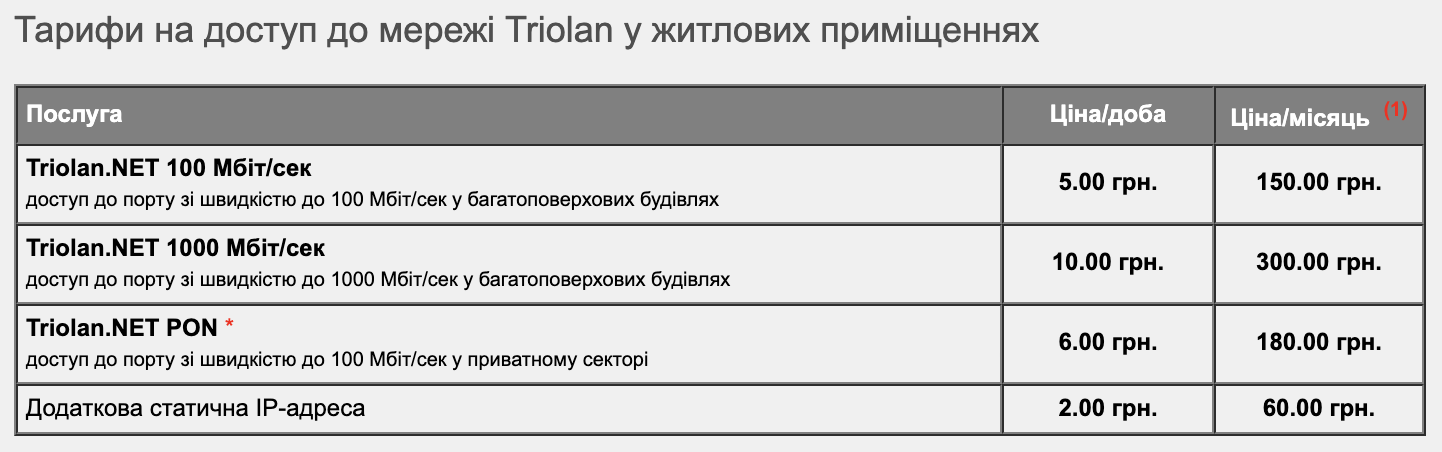
\includegraphics[width=0.8\textwidth]{triolan}
	\caption{Тарифні плани інтернет-провайдеру <<Тріолан>>~\cite{TriolanPrice}}
	\label{fig:triolan}
\end{figure} 

Витрати на інтернет доступ (рисунок~\ref{fig:triolan}):
\begin{gather*}
	C_{misc:triolan} = 150 * 6 * 18 = 16200 \textup{ грн.}
\end{gather*}

\subsection{Загальні витрати на проект}
Результати загальних розрахунків витрат на проект зведені у таблицю~\ref{tab:economy_total}.

{
	\tabulinesep=1.2mm
	\begin{longtabu} to \textwidth {|X[4,l]|X[1,l]|}
		\caption{Загальні витрати}
		\label{tab:economy_total} \\
		\hline
		Найменування витрат & Витрати \\
		\hline
		\endfirsthead
		\caption*{Закінчення таблиці \thetable{}}\\
		\hline
		Найменування витрат & Витрати \\
		\hline
		\endhead

		Апаратне забезпечення & $230894$ грн. \\ \hline
		Оплата праці & $776560$ грн. \\ \hline
		Програмне забезпечення & $107834.4$ грн. \\ \hline
		Зовнішні постачальники послуг & $16200$ грн. \\ \hline
		$\sum$ & $1131488.4$ грн. \\ \hline
	\end{longtabu}
}

В даному розділі було виконано розрахунки собівартості на розробку \acrshort{sw} для аналізу стійкості функціонування логістичних систем. В результаті було отримано, що на виконання робіт по розробці буде витрачено півтора року та повна собівартість $1131488.4$ грн. Собівартість складається з витрат на апаратне забезпечення, програмне забезпечення, заробітну плату та витрат на зовнішніх постачальників послуг.

% \section{Охорона праці і навколишнього середовища}
\subsection{Аналіз умов праці на робочому місці}
Розділ виконано для етапу розробки на ЕОМ MacBook Pro (15-inch, 2018).

Робота проводилась на кафедрі <<Програмної інженерії та Інформаційних Технологій Управління>>, яка розташована на сьомому поверсі семи поверхової будівлі.

Обладнання, приміщення і режим праці користувача повинні відповідати вимогам наступних нормативно-технічних документів:
\begin{enumerate}
	\item НПАОП 0.00-7.15-18. Вимоги щодо безпеки та захисту здоров’я працівників під час роботи з екранними пристроями.
	\item ДСанПіН 3.3.2.007-98. Державні санітарні правила і норми роботи з візуальними дисплейними терміналами електронно-обчислювальних машин.
	\item ДСТУ Б В.1.1-36:2016. Визначення категорій приміщень, будинків та зовнішніх установок за вибухопожежною та пожежною небезпекою.
	\item ДБН В.1.1-7-2016. Пожежна безпека об’єктів будівництва. Загальні вимоги.
	\item ДСН 3.3.6.042-99. Санітарні норми мікроклімату виробничих приміщень.
	\item ДБН В.2.5-67:2013. Опалення, вентиляція та кондиціонування.
	\item ДБН В.2.5-28-2018. Природне та штучне освітлення.
	\item ДСН 3.3.6.037-99. Санітарні норми виробничого шуму, ультразвуку та інфразвуку.
	\item ГОСТ 12.1.029-80 ССБТ. Средства и методы защиты от шума. Классификация.
	\item ДСТУ ГОСТ 12.1.012:2008. Вібраційна безпека. Загальні вимоги.
	\item ДСН 3.3.6.039-99. Санітарні норми виробничої загальної та локальної вібрації.
	\item ДСТУ ГОСТ 2656885:2009. Вібрація. Методи і засоби захисту. Класифікація.
	\item ДСТУ ГОСТ 12.1.038:2008. Електробезпека. Гранично допустимі рівні напруг дотику і струмів.
	\item ПУЕ. Правила улаштування електроустановок.
	\item НПАОП 40.1-1.32-01. Правила будови електроустановок. Електрообладнання спеціальних установок.
	\item ДСТУ ГОСТ 7237:2011. Електробезпека. Загальні вимоги та номенклатура видів захисту.
	\item ГОСТ 14254-96. Степени защиты, обеспечиваемые оболочками.
	\item НАПБ А.01.001-2014. Правила пожежної безпеки в Україні.
	\item ДСТУ БВ.2.5-38:2008. Інженерне обладнання будинків і споруд. Улаштування блискавка захисту будівель і споруд (IEC 62305:2006, NEQ).
	\item НАПБ Б.06.004-2005. Перелік однотипних за призначенням об’єктів, які підлягають обладнанню автоматичними установками пожежа гасіння та пожежної сигналізації.
	\item ГН 3.3.5-8.6.6.1-2014. Гігієнічна класифікація праці за показниками шкідливості та небезпечності факторів виробничого середовища, важкості та напруженості трудового процесу.
\end{enumerate}

Загальна характеристика виробничого приміщення, в якому виконувалась робота, приведена у таблиці~\ref{tab:labor_1}.

В таблиці~\ref{tab:labor_2} надано перелік потенційних небезпечних та шкідливих факторів на робочому місці користувача ЕОМ з монітором на рідинних кристалах.

\subsection{Захист від шкідливого впливу факторів виробничого середовища}
Захист від шкідливого впливу факторів виробничого середовища
Підтримка оптимальних параметрів мікроклімату в робочій зоні здійснюється відповідно вимог ДБН В.2.5-67:2013 за допомогою кондиціонеру, який регулює температуру повітря. Передбачена можливість природнього провітрювання приміщення. У холодний період року проводиться опалення від центральної тепломережі.%~\cite{Labor29}.

{
\footnotesize
\tabulinesep=1.2mm
\begin{longtabu} to \textwidth {|X[1,l]|X[3,l]|X[3,l]|X[3,l]|X[3,l]|X[3,l]|}
	\caption{Характеристика виробничого приміщення }
	\label{tab:labor_1} \\
	\hline
	№ п/п & Найменування показника & Характеристика показника & Обґрунтування вибору значення показника & Документ, що регламентує цій показник & Примітка \\
	\hline
	\endfirsthead
	\caption*{Закінчення таблиці \thetable{}}\\
	\hline
	№ п/п & Найменування показника & Характеристика показника & Обґрунтування вибору значення показника & Документ, що регламентує цій показник & Примітка \\
	\hline
	\endhead

	1 & 2 & 3 & 4 & 5 & 6 \\ \hline

	\multirow{2}{*}{1} & Розміри приміщення (м); & 4х5,3х3,3 & \multirow{2}{=}{На одне р.м. з ЕОМ не менше 6.0 $\textup{м}^2$ площі} & \multirow{2}{=}{ДСанПіН 3.3.2-007-98} & \multirow{2}{=}{Фактично 2.5-3 $\textup{м}^2$ на одне р.м. з ЕОМ, що відповідає нормі} \\ \cline{2-3}
	& Кількість робочих місць (р.м.) & 8 & & & \\ \hline

	\multirow{3}{*}{2} & \multirow{2}{=}{Природне освітлення, вікна виходять на південний схід} & \multirow{2}{=}{Бокове, одностороннє; азимут 135˚} &  Див. таблицю~\ref{tab:labor_2} & ДБН В.2.5-28-18 & \\ \cline{4-6}
	& & & КПО не нижче 1.5\% & ДСанПіН 3.3.2-007-98 & Для р.м. з ЕОМ \\
	& & & & &  \\ \hline

	\multirow{2}{*}{3} & \multirow{2}{=}{Штучне освітлення, кількість світильників N;  джерела світла} & \multirow{2}{=}{Загальне рівномірне; N=5; люмінесцентні лампи} & Див. таблицю~\ref{tab:labor_2} & ДБН В.2.5-28-18	& \\ \cline{4-6}
	& & & Не нижче 300-500 лк & ДСанПіН 3.3.2-007-98 & Для робочих місць з ЕОМ \\
	& & & & &  \\
	& & & & &  \\ \hline

	4 & Характеристика трифазної електричної мережі & Чотири провідна з глухо заземленою нейтраллю напругою 380/220 В, частотою 50 Гц & Довгі кабельні мережі великої ємності & ПУЕ & \\ \hline

	5 & Клас приміщення за ступенем небезпеки ураження електрострумом & З підвищеною небезпекою & Є можливість одночасного дотику до металоконструкцій будівлі, що мають з'єднання з землею, та до металевих корпусів ЕОМ & ПУЕ & Необхідно передбачити заходи безпеки згідно вимог ПУЕ \\ \hline

	6 & Категорія приміщення з вибухо-пожежної небезпеки & В & Є тверді спаленні матеріали: папір, деревина тощо & ДСТУ Б В.1.1-36:2016 & \\ \hline

	7 & Ступінь вогнестійкості будівельних конструкцій & ІІ & 7-и поверхова будівля; категорія В & ДБН В.1.1.7−2016	& \\ \hline

\end{longtabu}
}

{
\footnotesize
\tabulinesep=1.2mm
\begin{longtabu} to \textwidth {|X[1,l]|X[3,l]|X[3,l]|X[3,l]|X[3,l]|X[3,l]|}
	\caption{Перелік потенційних шкідливих та небезпечних факторів на робочому місці користувача ЕОМ з ЖК монітором}
	\label{tab:labor_2} \\
	\hline
	№ & Назва фактора & Джерела виникнення & Умови роботи & Нормативні параметри, їх значення & Документ, що регламентує показник \\
	\hline
	\endfirsthead
	\caption*{Закінчення таблиці \thetable{}}\\
	\hline
	№ & Назва фактора & Джерела виникнення & Умови роботи & Нормативні параметри, їх значення & Документ, що регламентує показник \\
	\hline
	\endhead

	1 & 2 & 3 & 4 & 5 & 6 \\ \hline

	\multicolumn{6}{|l|}{І. Небезпечні фактори} \\ \hline

	1 & Висока електрична напруга & Мережа живлення устаткування & Нормальний режим роботи & Струм $I_h = 0.3$ мА; Напруга $U_{\textup{дот}} < 2 \textup{В}$ & ДСТУ ГОСТ 12.1.038:08 \\ \hline

	\multicolumn{6}{|l|}{ІІ. Шкідливі фізичні фактори} \\ \hline

	2 & Несприятливе освітлення & Стан систем природного та штучного освітлення & МРОР 0,3-0,5 мм; розряд ІІІ; підрозряд <<в>>, фон середній, контраст середній & КПО $D_{\min}^{\textup{н сум}} = 1.2\%$; освітленість $E_{\min} = 300 \textup{лк}$ & ДБН В.2.5-28-18 \\ \hline

	3 & Несприятливий мікроклімат: температура ($t$), відносна вологість ($\phi$), швидкість руху ($v$) & Стан систем опалення та вентиляції & Категорія важкості робіт Іа; холодний період & Оптимальні:
	$t$ -- 22-24˚C;
	$\phi$ -- 40-60\%;
	$v$ -- не більше 0.1 м/с & ДСН 3.3.6.042-99 \\ \hline

	4 & Підвищений рівень шуму & Кондиціонери кулери, системи освітлювання, перетворювачі напруги, принтери & Творча діяльність, програмування & Рівень звуку $L_A = 50\textup{ дБА}$ & ДСН 3.3.6.037-99 \\ \hline

	5 & Вібрація & & Загальна технологічна, категорія 3, тип <<в>>, умови комфорту & Рівень віброшвидкості $L_V = 75\textup{ дБ}$ & ДСТУ ГОСТ 12.1.012:08, ДСН 3.3.6.039-99 \\ \hline

	6 & Психо-фізіологічна перенапруга & Монотонність праці, розумова напруга, статичність і незручність пози & & 1 та 2 клас умов праці для напруженості і важкості трудового процесу & ГН 3.3.5-8.6.6.1-2014 \\ \hline

\end{longtabu}
}

Згідно ДСН 3.3.6.042-99, у приміщеннях із значними площами засклених поверхонь передбачаються заходи щодо захисту:
\begin{itemize}
	\item від перегрівання при попаданні прямих сонячних променів в теплий період року (орієнтація віконних прорізів схід -- захід, улаштування лоджій, жалюзі, сонцезахисних плівок та інше);
	\item від радіаційного охолодження --- в зимовий (використання стін певної товщини, подвійних стекол).
\end{itemize}

Робочі місця повинні бути віддалені від стін на відстань не менше 1 м.

Визначений в таблиці~\ref{tab:labor_2} коефіцієнт природного освітлення реалізується через вікна визначеної площини, яка розраховується при проектуванні будівлі, а нормований показник штучного освітлення ($E_{\min}$) реалізується шляхом встановлення визначеної кількості світильників і вибором потужності ламп в них.

Згідно вимог ДСанПіН 3.3.2.007-98, в разі штучного освітлення як джерела світла мають застосовуватись переважно люмінісцентні лампи типу ЛБ і світильники серії ЛПО3б із дзеркальними гратами, укомплектовані високочастотними пускорегулювальними апаратами (ВЧ ПРА).

Система загального освітлення має становити суцільні або преривчасті лінії світильників, розташовані збоку від робочих місць (переважно ліворуч), паралельно лінії зору працюючих. Слід передбачити обмеження прямої блискості від джерел природного та штучного освітлення та обмежувати відбиту блискість на робочих поверхнях. Необхідно чистити вікна і світильники не менше двох разів на рік та вчасно заміняти перегорілі лампи.%~\cite{Labor30}.

Заходи захисту від шуму та вібрації повинні відповідати вимогам ГОСТ 12.1.029-80 і ДСТУ ГОСТ 2656885:2009. Устаткування, що є джерелом шуму, слід розташовувати поза приміщенням для роботи з ЕОМ. Для забезпечення допустимих рівнів шуму у виробничих приміщеннях слід застосовувати засоби звукопоглинання, наприклад, перфоровані плити, панелі, підвісні стелі.

Як захист від шуму, який створюється вентиляторами системних блоків, використовується звукоізоляційний корпус. Вентилятор можна замінити на більш якісний або на мідні радіатори з водяним охолодженням. Крім того встановлюють перехідник з регулятором напруги і швидкості обертання процесорного кулеру, а при монтажі кулерів металеві гвинти заміняють гумовими пробками, що дозволяють ізолювати вентилятор від корпусу. Якщо принтер розташований на твердій поверхні, то для зменшення вібрації потрібно підстелити під нього щільний прогумований килимок.

\subsection{Електробезпека}
Персональна ЕОМ є однофазним споживачем електроенергії, який живиться від трифазної чотирьох провідної мережі перемінного струму напругою 380/220 В частотою 50 Гц з глухо заземленою нейтраллю.

У разі випадкового дотику до струмопровідних частин, що знаходяться під напругою, або появі напруги дотику на металевих кожухах електроустаткування, наприклад, при пошкодженні ізоляції можливі нещасні випадки в результаті дії електричного струму.

Клас пожежа небезпечної зони приміщення, згідно ПУЕ та НПАОП 40.1-1.32-01, −П-ІІа, бо у приміщенні знаходяться тверді спаленні матеріали.

Для приміщень з підвищеною небезпекою поразки людини електричним струмом ПУЕ передбачені конструктивні, схемно-конструктивні й експлуатаційні міри електробезпеки (ДСТУ ГОСТ 7237:2011):%~\cite{Labor31}:
\begin{itemize}
	\item Експлуатаційні міри. Необхідно дотримуватися правил безпеки при роботі з високою напругою і використовувати наступні запобіжні заходи, що передбачені НПАОП 0.00-7.15-18: не підключати і не відключати кабелю, якщо обладнання знаходиться під напругою; технічне обслуговування і ремонтні роботи виконувати тільки при вимкнутому живленні в мережі; встановлювати у приміщенні загальний вимикач для відключення електроустаткування. Забороняється залишати працюючу апаратуру без нагляду.
	\item Конструктивні заходи. ЕОМ відноситься до електроустановок до 1000 В закритого виконання, усі струмоведучі частини знаходяться в кожухах. Вибираємо ступінь захисту оболонки від зіткнення персоналу із струмоведучими частинами усередині захисного корпуса і від потрапляння води усередину корпусу ІP-44, де перша <<4>> --- захист від твердих тіл, розміром більш 1.0 мм, друга <<4>> --- захист від бризків води (ГОСТ 14254-96).
	\item Як схемно-конструктивна міра безпеки застосовується подвійна ізоляція (для монітору), малі напруги до 42 В, занулення (так як мережа живлення до 1000 В з глухо заземленою нейтраллю). Відповідно ДСТУ ГОСТ 7237:2011, занулення --- це навмисне електричне з'єднання металевих неструмоведучих частин комп'ютера, які у випадку аварії можуть виявитися під напругою, з нульовим захисним провідником.
\end{itemize}

Вихідні дані для розрахунку занулення однофазних споживачів (варіант 24):
\begin{equation*}
	P_1 = 525\textup{ Вт}, P_2 = 16000\textup{ Вт},
\end{equation*}
\begin{description}
	\item[де] $P_1$ --- потужність однофазного споживача електроенергії, наприклад, електронно-обчислювальної машини (ЕОМ), Вт;
	\item $P_2$ --- потужність усіх споживачів, які живляться від цього фазового провідника (кондиціонери, вентилятори, освітлювальні прилади, інші ЕОМ, принтери, тощо), кВт.
\end{description}
\begin{equation*}
	l_1 = 55\textup{ м}, l_2 = 138\textup{ м},
\end{equation*}
\begin{description}
	\item[де] $l_1$ --- довжина ділянки 1, м;
	\item $l_2$ --- довжина ділянки 2, м.
\end{description}
\begin{equation*}
	U_{\textup{л}} = 380\textup{ В}, U_{\textup{ф}} = 220\textup{ В},
\end{equation*}
\begin{description}
	\item[де] $U_{\textup{л}}$ --- лінійна напруга;
	\item $U_{\textup{ф}}$ --- фазова напруга.
\end{description}

Матеріал провідників -- алюміній, спосіб прокладки проводів на ділянці 1 -- металеві труби, на ділянці 2 -- земля. 

Занулення використовується в чотири провідних трифазових мережах із заземленою нейтраллю напругою до 1000 В. 
Схема мережі до розрахунку занулення зображена на рис.~\ref{fig:labor_nullation}.

\begin{figure}[H]
	\centering
	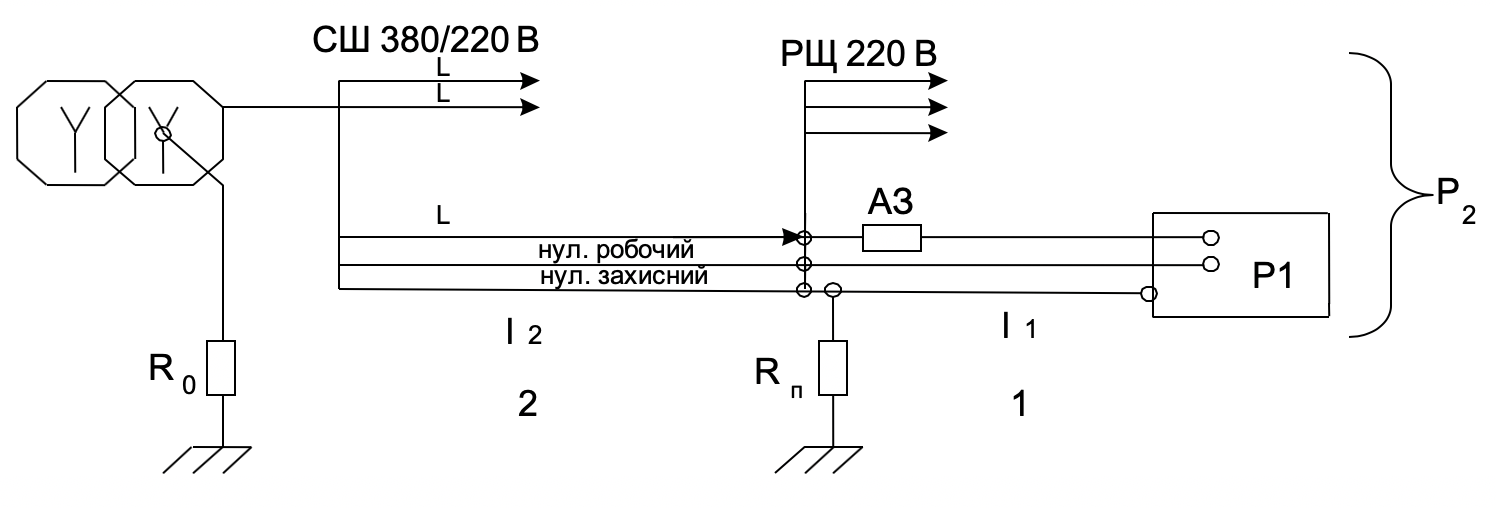
\includegraphics[width=0.8\textwidth]{labor_nullation}
	\caption{Схема мережі до розрахунку занулення}
	\label{fig:labor_nullation}
\end{figure}
\begin{description}
	\item[де] $T_{\textup{р}}$ --- масляний трансформатор, що понижує напругу з $U_1 = 6-10$ кВ до $U_2 = 380$ В, схема з'єднання обмоток --- зірка-зірка;
	\item ЗШ --- збірна шина;
	\item РЩ --- розподільний щит;
	\item АЗ --- апарат захисту;
	\item 1 --- лінія, що живить електроустановку потужністю $Р_1$;
	\item 2 --- живильний магістральний кабель.
\end{description}

Мета розрахунку --- визначення такого перерізу нульового захисного провідника, при якому струм короткого замикання (ІК) у задане число разів (К) перевищить номінальний струм апарату захисту ($I^{\textup{АЗ}}_{\textup{НОМ}}$), що забезпечить селективне відключення споживача, тобто повинна виконуватися умова:
\begin{equation} \label{eq:lab_check}
	I_{\textup{К}} \geq K \cdot I^{\textup{АЗ}}_{\textup{НОМ}}.
\end{equation}
\begin{description}
	\item[де] $K$ --- запас надійності.
\end{description}

Електромережа, що живіть комп'ютер та інші однофазні електроустановки, виконується як групова три провідна лінія шляхом прокладання фазового, нульового робочого і нульового захисного провідників з міді або алюмінію. Якщо кількість ЕОМ не перевищує 5 і вони розташовані по периметру приміщення, кабель в оболонці з неспалених матеріалів прокладають по підлозі вздовж стін. Якщо кількість ЕОМ перевищує 5 або вони розташовані у центрі приміщення, кабель прокладають у металевих трубах та гнучких металевих рукавах з відводами.

Нехай струм $I_1$, що живить електроустановку (ЕУ) потужністю $Р_1$, Вт:
\begin{equation*}
	I_1 = \cfrac{P_1}{U_{\textup{ф}}} = \cfrac{525}{220} = 2.3863, \textup{A}.
\end{equation*}

Струм $I_2$, що живить електроустановку (ЕУ) потужністю $Р_2$, Вт:
\begin{equation*}
	I_2 = \cfrac{P_2}{U_{\textup{ф}}} = \cfrac{16000}{220} = 72.7272, \textup{A}.
\end{equation*}

Визначення пускового струму $I_{\textup{пуск}}$ потужністю $P_1$, Вт:
\begin{equation*}
	I_{\textup{пуск}} =\cfrac{K_n}{K_T} I_1, \textup{A}.
\end{equation*}
\begin{description}
	\item[де] $K_n$ --- коефіцієнт кратності пускового струму, 2\dots7.5;
	\item $K_T$ --- коефіцієнт важкості пуску, залежить від часу пуску, 1.6\dots2.5; $K_T = 1.6$, якщо час пуску понад 10 с --- тяжкий пуск; $K_T = 1.6$, якщо час пуску дорівнює 10 с --- середній пуск; $K_T = 2.5$ якщо час пуску дорівнює 5 с --- легкий пуск.
\end{description}

Для ЕОМ $K_n = 3, K_T = 2.5$, тоді:
\begin{equation*}
	I_{\textup{пуск}} =\cfrac{3}{2.5} 2.3863 = 2.8635, \textup{A}.
\end{equation*}

Номінальний струм, при якому спрацьовує апарат захисту, повинен перевищувати $І_\textup{пуск}$, інакше апарат захисту буде спрацьовувати при кожному вмиканні електроустановки.

Для ЕОМ можна вибрати запобіжник типу ВПШ. Згідно із розрахунків $I_{\textup{пуск}}$, можна використовувати ВПШ значення якого вище $2.8635$ А, а саме ВПШ 6-11 з $I^{\textup{АЗ}}_{\textup{НОМ}} = 3.15$ А.

Струм короткого замикання $I_\textup{к}$, визначаємо за формулою:
\begin{equation} \label{eq:lab_ik}
	I_\textup{к} = \cfrac{U_\textup{ф}}{
		\cfrac{Z_{TP}}{3} + Z_{\textup{ПФН}}
	}, \textup{А},
\end{equation}
\begin{description}
	\item[де] $Z_{TP}$ --- повний опір трансформатора, Ом;
	\item $Z_{\textup{ПФН}}$ --- повний опір петлі фаза-нуль, Ом.
\end{description}

Величина $Z_{TP}$ залежить від потужності трансформатора, конструктивного виконання, напруги і схеми з¢єднання його обмоток (зіркою або трикутником).

Потужність трансформатора визначається за формулою:
\begin{equation*}
	N_{TP} = 4 \cdot P_2 = 4 \cdot 16 = 64, \textup{кВт}.
\end{equation*}

Вибираємо трансформатор потужністю 100 кВт, $Z_{TP} = 0.799$ Ом.

Повний опір петлі фаза-нуль визначається за формулою:
\begin{equation*}
	Z_{\textup{ПФН}} = \sqrt{(R_\textup{Ф} + R_\textup{НЗ})^2 + X^2}, \textup{Ом},
\end{equation*}
\begin{description}
	\item[де] $R_\textup{Ф}$ --- активний опір фазового захисного провідника, Ом;
	\item $R_\textup{НЗ}$ --- активний опір нульового захисного провідника, Ом.
\end{description}

Індуктивний опір петлі фаза-нуль $X$ визначається за формулою:
\begin{equation*}
	X = X_\textup{Ф} + X_\textup{НЗ} + X_\textup{ВЗ}, \textup{Ом},
\end{equation*}
\begin{description}
	\item[де] $X_\textup{Ф}$, $X_\textup{НЗ}$ --- внутрішні індуктивні опори фазового і нульового провідників, відповідно, Ом;
	\item $X_\textup{ВЗ}$ --- зовнішній індуктивний опір, який зумовлено взаємоіндукцією петлі фаза-нуль, Ом.
\end{description}

Для мідних та алюмінієвих провідників $X_\textup{Ф}$ та $X_\textup{НЗ}$ порівняно малі (близько $0.0156$ Ом/км), тому ними можна знехтувати.

Зовнішній індуктивний опір $X_\textup{ВЗ}$ залежить від відстані між проводами $D$ та їхнього діаметру $d$. Якщо нульові захисні проводи прокладають спільно з фазовими, значення $D$ мале й порівняльне з діаметром $d$, тому опір $X_\textup{ВЗ}$ незначний (не більш $0.1$ Ом/км) і ним можна знехтувати. Тоді:
\begin{equation*}
	Z_{\textup{ПФН}} = R_\textup{Ф} + R_\textup{НЗ}.
\end{equation*}

Таким чином первинна формула розрахунку~\eqref{eq:lab_ik} приймає вид:
\begin{equation*}
	I_\textup{к} = \cfrac{U_\textup{ф}}{
		\cfrac{Z_{TP}}{3} + R_\textup{Ф} + R_\textup{НЗ}
	}, \textup{А},
\end{equation*}

Визначимо значення активного опору фазового провідника за формулою:
\begin{equation} \label{eq:lab_r}
	R_{\textup{Ф}} = R_\textup{Ф1} + R_\textup{Ф2},
\end{equation}
\begin{description}
	\item[де] $R_\textup{Ф1}$, $R_\textup{Ф2}$ --- опір фазового провідника на ділянках 1 та 2, відповідно, Ом.
\end{description}

Для провідників з кольорових металів:
\begin{equation*}
	R_{\textup{Ф1}} = \cfrac{\rho\cdot l_1}{S_\textup{Ф1}}, \textup{Ом},
\end{equation*}
\begin{equation*}
	R_{\textup{Ф2}} = \cfrac{\rho\cdot l_2}{S_\textup{Ф2}}, \textup{Ом},
\end{equation*}
\begin{description}
	\item[де] $\rho$ --- питомий опір, $\cfrac{\textup{Ом} \cdot \textup{мм}^2}{\textup{м}}$, який дорівнює для міді $0.018$, а для алюмінію $0.028$;
	\item $S_\textup{Ф1}$, $S_\textup{Ф2}$ --- перерізи фазового провідника для ділянок 1 та 2, відповідно, $\textup{мм}^2$.
\end{description}

Перерізи фазових проводів визначають при проектуванні електричної мережі струму в залежності від величини струму, який проходить по проводам, умов прокладання кабелю, матеріалу провідників і т.п. Так згідно із вихідними даними значення перерізів дорівнюють:
\begin{equation*}
	S_{\textup{Ф1}} \approx 2, S_{\textup{Ф2}} \approx 7.
\end{equation*}

Опір фазових провідників дорівнюють:
\begin{equation*}
	R_{\textup{Ф1}} = \cfrac{\rho\cdot l_1}{S_\textup{Ф1}} = \cfrac{0.028 \cdot 55}{2} = 0.77, \textup{Ом},
\end{equation*}
\begin{equation*}
	R_{\textup{Ф2}} = \cfrac{\rho\cdot l_2}{S_\textup{Ф2}} = \cfrac{0.028 \cdot 138}{7} = 0.552, \textup{Ом}.
\end{equation*}

Визначення опору нульового захисного провідника:
\begin{equation*}
	R_{\textup{НЗ}} = R_{\textup{НЗ1}} + R_{\textup{НЗ2}}, \textup{Ом},
\end{equation*}
\begin{description}
	\item[де] $R_{\textup{НЗ1}}$, $R_{\textup{НЗ2}}$ --- опір нульового захисного провідника на ділянках 1 та 2, відповідно, Ом.
\end{description}

Площа перерізу нульового робочого та нульового захисного провідників в груповій три провідній мережі повинна бути не менш площі фазового провідника, тобто: $S_\textup{НЗ1} = S_\textup{Ф1}$, $S_\textup{НЗ2} = S_\textup{Ф2}$.
Відповідно, $S_\textup{НЗ} = S_\textup{Ф}$.

Обчислимо опір фазового провідника~\eqref{eq:lab_r}:
\begin{equation*}
	R_{\textup{НЗ}} = R_{\textup{Ф}} = R_{\textup{Ф1}} + R_{\textup{Ф2}} = 1.322, \textup{Ом},
\end{equation*}
отже:
\begin{equation*}
	I_\textup{к} = \cfrac{220}{
		\cfrac{0.799}{3} + 1.322 + 1.322
	} = \cfrac{220}{2.9103} = 75.5927, \textup{А}.
\end{equation*}

Перевірка виконання умов надійності та ефективності роботи занулення.
Повинно виконуватися співвідношення~\eqref{eq:lab_check}, де $K = 3$ для запобіжників:
\begin{equation*}
	75.5927 \geq 3 \cdot 3.15.
\end{equation*}

Утрати напруги на ділянках 1 та 2 не повинні перебільшувати 22 В:
\begin{gather*}
	U_\textup{П1} + U_\textup{П2} \leq 22, \textup{В}, \\
	U_\textup{П1} = I_1 \cdot R_\textup{Ф1} = 2.3863 \cdot 0.77 = 1.8374, \textup{В}, \\
	U_\textup{П2} = I_2 \cdot R_\textup{Ф2} = 72.7272 \cdot 0.552 = 40.1454, \textup{В}, \\
	40.1454 + 1.8374 \leq 22.
\end{gather*}

Виходячи з розрахунків, друга умова не виконується і треба обрати більше значення для перерізу фазового провідника для ділянки 2, так як вона має велику утрату напруги.

Беручи $S_\textup{Ф2} = 14$ повторимо розрахунки:
\begin{gather*}
	R_{\textup{Ф2}} = \cfrac{\rho\cdot l_2}{S_\textup{Ф2}} = \cfrac{0.028 \cdot 138}{14} = 0.276, \textup{Ом}, \\
	U_\textup{П2} = I_2 \cdot R_\textup{Ф2} = 72.7272 \cdot 0.276 = 20.0727, \textup{В}, \\
	20.0727 + 1.8374 \leq 22.
\end{gather*}

Всі умови виконуються. Таким чином були обрані:
\begin{itemize}
	\item запобіжник ВПШ 6-11;
	\item перерізи фазового та нульового захисного провідників для першої ділянки 2 $\textup{мм}^2$;
	\item перерізи фазового та нульового захисного провідників для першої ділянки 14 $\textup{мм}^2$.
\end{itemize}

\subsection{Пожежна безпека}
У зв'язку з поширенням комп’ютерної техніки, що може привести до загоряння, треба передбачати можливі наслідки і розробляти заходи щодо їх попередження. Причинами загоряння стають: несправність електричного обладнання, пошкодження ізоляції, коротке замикання кола струму, перегрів проводів, поганий контакт в місцях з'єднання; розряди статичної електрики, які особливо небезпечні в вибухонебезпечних приміщеннях, блискавка.

Пожежна безпека забезпечується наступними мірами:
\begin{enumerate}[label={\arabic*)}]
	\item системою запобігання пожеж;
	\item системою пожежного захисту;
	\item організаційними заходами щодо пожежної безпеки.
\end{enumerate}

Система запобігання пожеж передбачає запобігання утворенню пального середовища і запобігання утворенню в пальному середовищі джерел запалювання.

Для зменшення небезпеки утворення в пальному середовищі джерел запалювання передбачено:
\begin{enumerate}[label={\arabic*)}]
	\item використання електроустаткування, що відповідає класу пожежа небезпечної зони приміщення П-ІІа за ПУЕ та НПАОП 40.1-1.32-01: ступінь захисту електроапаратури не менш ІP-44, ступінь захисту світильників ІР-2Х;
	\item використання електроустаткування, що відповідає класу пожежа небезпечної зони приміщення П-ІІа за ПУЕ та НПАОП 40.1-1.32-01: ступінь захисту електроапаратури не менш ІP-44, ступінь захисту світильників ІР-2Х;
	\item забезпечення захисту від короткого замикання (контроль і профілактика ізоляції, використання запобіжників);
	\item вибір перетину провідників по максимально допустимому нагріванню;
	\item будівлі, в яких встановлено обладнання інформаційних технологій чи будь-яке інше електронне обладнання, чутливе до атмосферних перешкод, незалежно від кількості уражень об'єктів за рік потребує І або ІІ рівня блискавка захисту (ДСТУ БВ.2.5-38:2008).
\end{enumerate}

Система протипожежного захисту призначена для локалізації та гасіння пожежі. При виборі засобів гасіння пожежі для забезпечення безпеки людини від можливості поразки електричним струмом у приміщенні відповідно вимог НАПБ А.01.001-2014 передбачено використання вуглекислотних вогнегасникiв ВВК-5. Вогнегасник знаходиться на видному і легко доступному місці. При виникненні пожежі передбачені можливості аварійного відключення апаратури і комунікацій та повідомлення в пожежну охорону по телефону. У якості сповіщувачів використовуються система автоматичної пожежної сигналізації відповідно вимог НАПБ Б.06.004-2005. Ступінь вогнестійкості будинку згідно ДБН В.1.1-7-2016 --- ІІ. У приміщенні є два незалежних виходи для евакуації людей під час пожежі.

Організаційними заходами протипожежної профілактики є вступний інструктаж при надходженні на роботу, навчання виробничого персоналу протипожежним правилам, видання необхідних інструкцій і плакатів, засобів наочної агітації, наявність плану евакуації.%~\cite{Labor32}.

\subsection{Охорона навколишнього середовища}
Закон України <<Про охорону навколишнього середовища>> від 25 червня 1991р. --- закон, що визначає правові, економічні та соціальні основи організації охорони природи навколишнього природного середовища в інтересах нинішнього і майбутніх поколінь.

Закон встановлює, що завданням законодавства про охорону навколишнього природного середовища є регулювання відносин у галузі охорони, використання і відтворення природних ресурсів, забезпечення екологічної безпеки, запобігання і ліквідації негативного впливу господарської та іншої діяльності на навколишнє природне середовище, збереження природних ресурсів, генетичного фонду живої природи, ландшафтів та інших природних комплексів, унікальних територій та природних об'єктів, пов'язаних з історико-культурною спадщиною.

Збільшення використання енергії призводить до порушення екологічної рівноваги природного середовища, яке складалася століттями. 

Поряд з цим, підвищення технічної оснащеності підприємств, застосування нових матеріалів, конструкцій і процесів, збільшення швидкостей і потужностей виробничих машин впливають на навколишнє середовище.

При масовому використанні моніторів та комп’ютерів не можна не враховувати їхній вплив на навколишнє середовище на всіх стадіях --- при виготовленні, експлуатації та після закінчення терміну служби.

Міжнародні екологічні стандарти, що діють на сьогоднішній день в усьому світі, визначають набір обмежень до технологій виробництва та матеріалів, які можуть використовуватися в конструкціях пристроїв. Так, за стандартом ТСО-95, вони не повинні містити фреонів (турбота про озоновий шар), полівінілхлориді, бромідів (як засобів захисту від загоряння).

У стандарті ТСО-99 закладене обмеження за кадмієм у світлочутливому шарі екрана дисплея та ртуті в батарейках; э чіткі вказівки відносно пластмас, лаків та покриттів, що використовуються. Поверхня кнопок не повинна містити хром, нікель та інші матеріали, які визивають алергічну реакцію. ГДК пилу дорівнює $0.15 \textup{мг/м}^3$, рекомендовано $0.075 \textup{мг/м}^3$; ГДК озону під час роботи лазерного принтеру --- $0.05 \textup{мг/м}^3$. Особливо жорсткі вимоги до повторно використовуваних матеріалів.

Міжнародні стандарти, починаючи з ТСО-92, включають вимоги зниженого енергоспоживання та обмеження припустимих рівнів потужності, що споживаються у неактивних режимах.
Дотримання приведених нормативних параметрів небезпечних і шкідливих виробничих факторів дозволить забезпечити більш здорові і безпечні умови роботи користувача ЕОМ.


\section*{Висновки}
\addcontentsline{toc}{section}{Висновки}
Сучасні алгоритми <<комп'юторного зору>> дозволяють досить швидко створювати вражаючі програми які реалізують зоровий інтерфейс.
Використання нейронних мереж спрощує задачу переведення точок обличчя у положення погляду не екрані.

В ході написання роботи дану задачу було розкрито повною мірою на прикладі проектування та реалізації програмної системи для визначення погляду користувача з видеоряду та керування курсором за допомогою погляду. 

В процесі дослідження були сформульовані вимоги до програмної системи, та обрана й спроектована її архітектура.
Обгрунтований вибір інструментальних засобів розробки.

\printbibliography[heading=bibintoc, title={Список джерел інформації}]


\begin{appendices}
	% custom commands 
	\newcommand\appendixsection[1]{
		\addtocounter{section}{1}
		\clearpage
		\begin{center}
		  \bfseries\centering
		  \MakeUppercase{Додаток \thesection}\\#1
		  \vspace*{0.1cm}
		\end{center}
		\addcontentsline{toc}{section}{Додаток \thesection. #1}
	}

	\appendixsection{Порівняння платформ для розробки мультагентних систем}
{
	\small
	\tabulinesep=1.2mm
	\begin{longtabu} to \textwidth {|X[2,l]|X[2,l]|X[3,l]|X[3,l]|}
  		\caption{Порівняння платформ для розробки \acrshort{mas}~\cite{Kravari2015}}
  		\label{tab:mas_platform_comparsion} \\
		\hline
		& \textbf{Agent Factory} & \textbf{\acrshort{jade}} & \textbf{AnyLogic} \\\hline\endfirsthead
  		\caption*{Продовження таблиці \thetable{}}\\
		\hline
		& \textbf{Agent Factory} & \textbf{\acrshort{jade}} & \textbf{AnyLogic} \\\hline\endhead
		% Platform properties
		Организація & University College Dublin & Telecom Italia (TILAB) & Компанія AnyLogic \\\hline
		Основна доменна область & Агенти для загального призначення & Розподілені мультиагентні системи & Розподілені мільтиагентні симуляції \\\hline
		Ліцензія & LGPL & LGPL & Комерційна та академічна ліцензії \\
		\hline
		% Usability overview
		Простота використання & Простий / Нестача функціоналу у \acrshort{gui} & Зручний, простий \acrshort{gui}, багато звичних функцій & Середній / Багатий функціонал \acrshort{gui} \\\hline
		Легкість вивчення платформи & Середня & Легка (багато прикладів) & Легка \\\hline
		Масштабованість & Добра & Висока & Висока \\\hline
		Сумісність зі стандартами & \acrshort{fipa} & \acrshort{fipa}, \acrshort{corba} & \acrshort{gis}, 3D-можливості \\
		\hline
		% Operating ability of each agent platform
		Продуктивність & Добра & Висока (дуже швидка взаємодія між агентами) & Висока \\\hline
		Надійність & Середня & Висока & Висока \\\hline
		Мови програмування & Java, \acrshort{afapl}, AgentSpeak & Java & Java, \acrshort{uml}-RT (\acrshort{uml} для реального часу) \\\hline
		Операційні системи & Будь-яка з \acrshort{jvm} & Будь-яка з \acrshort{jvm} & Будь-яка з \acrshort{jvm} \\
		\hline
		% Pragmatics overview
		Рівень підтримки & Добрий (документація, розсилка пошти, форум) & Високий (\acrshort{faq}, розсилка пошти, список дефектів, \acrshort{api}, документація) & Високий (документація) \\\hline
		Популярність & Низька & Висока (найпопулярніша платформа) & Середня \\\hline
		Зрілість технології & Стабільний випуск, статус розробки (неактивний) & Стабільний випуск, статус розробки (активний) & Стабільний випуск, статус розробки (активний) \\\hline
		Вартість & Безкоштовна & Безкоштовна & AnyLogic Advanced \$6,199, Professional \$15,800, University Researcher License \$3,500, Educational Licenses \$485 \\
		\hline
		% Security management overview
		Кінцевий рівень безпеки & Підпис і шифрування & Підпис і шифрування, підтримка HTTPS & Аутентифікація \\\hline
		Справедливість \textit{(fairness)} & Ні & Так & Так \\\hline
		Безпека платформи & Середня & Сильна (аутентифікація, Jaas \acrshort{api}) & Сильна (закрита система) \\
		\hline
	\end{longtabu}
}
\end{appendices}

\end{document}